\documentclass[12pt]{article}
\usepackage{graphicx}
\usepackage{parskip}
\usepackage{amsmath,amssymb}
\usepackage{hyperref}
\usepackage{fontspec}
\usepackage{setspace}
\usepackage[margin=1in]{geometry}
\usepackage[table,xcdraw]{xcolor}
\usepackage[textfont={rm,it}]{caption}
\usepackage{subcaption}
\usepackage{subfloat}
\usepackage{multirow}
\usepackage{multicol}
\usepackage[american]{babel}
\usepackage{csquotes}
\allowdisplaybreaks

\numberwithin{equation}{section}
\begin{document}
\title{Yizhong Hu Summer 2023 Results Report}
\author{Yizhong Hu}
\maketitle

\section{Jun 1 - Jun 5}

\subsection{Model Description}

We consider the Hamiltonian $\mathcal{H}: \mathcal{X}^{\kappa + 1} \times \mathcal{Y}^{\kappa} \mapsto \mathbb{R}$

\begin{equation*}
    \mathcal{H}(x_0, x_1, \ldots, x_\kappa, y_{01}, \ldots, y_{0\kappa} ) = \frac{\beta}{2}\sum_{i=1}^\kappa x_0x_iy_{0i} + Bx_0
\end{equation*}
where $x_0$ is spin state of the root node, $x_i$ is the spin state of the $i$-th leaf node, $y_{0i}$ is the interaction between
$0$ and $i$. All of them take values in $\mathcal{X} = \mathcal{Y} = \{-1, 1\}$.

When $\kappa=2$,
\begin{equation*}
    \mathcal{H}(x_0, x_1, x_2, y_{01}, y_{02} ) = \frac{\beta}{2}(x_0x_1y_{01} + x_0x_2y_{02}) + Bx_0
\end{equation*}

We define the state $s$ in state space $\mathbb{S} = \mathcal{X}^3 \times \mathcal{Y}^2$, and the random variable $S$ a random variable
on $\mathbb{S}$. Given $\eta$ the i.i.d Bernoulli(1/2) distribution on $\mathbb{S}$, we want to investigate the distribution $\mu(\cdot)$ that maximizes
\begin{equation*}
    \max_{\mu(\cdot)} \left\{\mathbb{E}_\mu[\mathcal{H}(S)] - \left[H(\mu \| \eta) + H(\mu_{01}\|\eta_{01} )\right]\right\}
\end{equation*}

\subsection{Analytical analysis}

First, we need to find the distribution $\mu: \mathcal{X}^3 \times \mathcal{Y}^2 \mapsto [0, 1]$. Since the input is discrete,
$\mu$ can be rewritten as a vector on $[0, 1]^{2^5}$. We will denote each component as $\mu(s)$, with $s\in \mathbb{S}$

The marginal distribution is therefore
\begin{equation*}
    \mu_{01}(y_{01}) = \sum_{x_1, x_2, x_3, y_{02} \in \{-1, 1\}} \mu(s)
\end{equation*}

Rewriting each term,
\begin{align*}
    \mathbb{E}_\mu[\mathcal{H}(S)] & = \sum_{s\in \mathbb{S}} \mu(s) \mathcal{H}(s)                                                 \\
    H(\mu \| \eta)                 & = \sum_{s\in \mathbb{S}} \mu(s) \log\frac{\mu(s)}{\eta(s)}                                     \\
    H(\mu_{01} \| \eta_{01})       & = \sum_{y_{01}\in \mathcal{Y}} \mu_{01}(y_{01}) \log\frac{\mu_{01}(y_{01})}{\eta_{01}(y_{01})}
\end{align*}
Note that since $\eta$ is uniform, the relative entropies can be written directly in terms of their entropies:
\begin{align*}
    H(\mu \| \eta)           & = H(\mu) - \log |\mathbb{S}| \\
    H(\mu_{01} \| \eta_{01}) & = H(\mu_{01}) - \log 2
\end{align*}
Rewriting the target,
\begin{equation*}
    \max_{\mu(\cdot)} \left[\sum_{s\in \mathbb{S}} \mu(s) \mathcal{H}(s) - \sum_{s\in \mathbb{S}} \mu(s) \log \mu(s) + \sum_{y_{01}\in \mathcal{Y}} \mu_{01}(y_{01}) \log\mu_{01}(y_{01})\right]
\end{equation*}

The corresponding Lagrange multiplier (constrained on $\mu$ being normalized) is
\begin{equation*}
    \mathcal{L} =\left[\sum_{s\in \mathbb{S}} \mu(s) \mathcal{H}(s) - \sum_{s\in \mathbb{S}} \mu(s) \log \mu(s) + \sum_{y_{01}\in \mathcal{Y}} \mu_{01}(y_{01}) \log\mu_{01}(y_{01})\right] + \lambda\left[\sum_{s\in \mathbb{S}} \mu(s) - 1\right]
\end{equation*}
taking the gradients gives
\begin{align}
    \frac{\partial \mathcal{L}}{\partial \mu(s)}  & = \mathcal{H}(s) - \log \mu(s) + \log \mu_{01}(y_{01}) + \lambda = 0 \\
    \frac{\partial \mathcal{L}}{\partial \lambda} & = \sum_{s\in \mathbb{S}} \mu(s) - 1 = 0
\end{align}
where $y_{01}$ in Eq.(1) represents the value of $y_{01}$ in $s$.

Eq.(1) gives the form of $\mu$ in terms of a conditional distribution, as seen below:
\begin{align*}
    \log \mu(s) - \log \mu_{01}(y_{01})  & = \mathcal{H}(s) + \lambda     \\
    \log \frac{\mu(s)}{\mu_{01}(y_{01})} & = \mathcal{H}(s) + \lambda     \\
    \frac{\mu(s)}{\mu_{01}(y_{01})}      & = e^\lambda e^{\mathcal{H}(s)}
\end{align*}
The left-hand side is a conditional distribution:
\begin{equation}
    \mathbb{P}_\mu (S = s | Y_{01} = y_{01}) = \frac1Z \exp\left[\frac{\beta}{2}(x_0x_1y_{01} + x_0x_2y_{02}) + Bx_0\right]
\end{equation}
for some $Z = e^{-\lambda} = $ normalizing constant.

Since $\frac{\partial \mathcal{L}}{\partial \mu(s)} = 0$ for all $\mu_{01}$ values, and all such optimum points form a connected curve,
we think that it is reasonable to hypothesize that any choice of $\mu_{01}$ satisfies optimality.
Since $y_{01}$ can only take two values, the distribution can be characterized by a single real value $\alpha$:
\begin{equation*}
    \mathbb{P}_\mu(Y_{01} = y_{01}) = \frac{e^{\alpha y_{01}}}{e^\alpha + e^{-\alpha}},
\end{equation*}
and the entire distribution becomes
\begin{equation*}
    \mu(s) = \frac1Z \exp\left[\frac{\beta}{2}(x_0x_1y_{01} + x_0x_2y_{02}) + Bx_0 + \alpha y_{01}\right]
\end{equation*}

\subsection{Numerical Analysis}

On the other hand, this problem can be solved numerically, formulated as a constrained optimization:

\begin{align*}
    \text{maximize}\quad   & \sum_{s\in \mathbb{S}} \mu(s) \mathcal{H}(s) - \sum_{s\in \mathbb{S}} \mu(s) \log \mu(s) + \sum_{y_{01}\in \mathcal{Y}} \mu_{01}(y_{01}) \log\mu_{01}(y_{01}) \\
    \text{subject to}\quad & \sum_{s\in\mathbb{S}} \mu(s) = 1
\end{align*}

Since entropy calculations really don't like getting negative values, we will represent $\mu$ as an exponential:
\begin{equation*}
    \mu(s) = e^{x(s)}
\end{equation*}
Note that since $\exp: \mathbb{R} \mapsto (0, \infty)$ is bijective, we do not lose any generality.

A proximal point optimization method will be used for the optimization. For the following optimization problem

$$\begin{aligned}
        \text{maximize}\quad   & f(\textbf{x})                        \\
        \text{subject to}\quad & \textbf{g}(\textbf{x}) = \textbf{0},
    \end{aligned}$$
we have the following iterative process to obtain an optimum:
$$\begin{aligned}
        \textbf{x}^{(t+1)}       & = \text{argmax}_{\text{x}} f(\text{x}) + \mathbf{\lambda}^{(t)} \cdot \textbf{g}(\textbf{x}) - \frac12 (\textbf{g}(\textbf{x}))^2 \\
        \mathbf{\lambda}^{(t+1)} & = \mathbf{\lambda}^{(t)} - \textbf{g}\left(\textbf{x}^{(t+1)}\right)                                                              \\
    \end{aligned}$$
The minimization on $\textbf{x}$ is done with the SciPy minimize. The code is provided in the notebook attached.

Results from numerical analysis confirm the results from analytical analysis. Aside from inaccuracies introduced by low value of $\mu_{01}(y_{01})$,
the conditional distribution given $Y_{01}$ matches the exponential distribution $\exp[\mathcal{H}(s)]$ to around $10^{-6}$ accuracy. Additionally,
any distribution on $Y_{01}$ can be optimal, which conforms with the analytical understanding.

\subsection{Correlation}

To see the correlation, we will try to calculate the Pearson coefficient for the pairs of random variables. We will test these on different choices of $\beta$ and $B$. To make sure that the results are accurate, we reduced the accuracy requirement to below $10^{-10}$.

\begin{itemize}
    \item For $Y^*_{01}$, and $X^*_{0}$, we can see that the Pearson coefficient is very close to $0$ except for when $B$ is much larger than $1$ and $Y^*_{01}$
          is skewed to one of the results, which could be just an accuracy issue. We hence hypothesize that $Y^*_{01}$, and $X^*_{0}$ are independent.
          To make it more certain, we can try numerically calculating the distribution in exponential form to confirm.
\end{itemize}




It is unclear what correlation is like in this situation. Given how the distribution is structured, we can separate the exponent additively to obtain
mutually independent pieces. For example, if we fix $x_0$, we know that $X_1, Y_{01}$ and $X_2, Y_{02}$ are independent of each other:
\begin{equation*}
    \mu(s) = \frac1Z \exp(Bx_0) \exp\left[\frac{\beta}{2}(x_0x_1y_{01}) + \alpha y_{01}\right] \exp\left[ \frac\beta2 x_0x_2y_{02}\right]
\end{equation*}
I have tried to calculate the covariance between different random variables from the numerical results, but they differ by the choice of $\mu_{01}$,
and the marginal distributions don't seem like there is a definitive answer for if they correlate or are independent. I may need more guidance on this
issue.

\newpage

\section{Jun 6 - Jun 12}

To simplify, we still consider the Ising model.

\subsection{Numerical Analysis}

\subsubsection{Method}

We vectorize the state, representing the probability as $\mu_{x_0k}$, where $x_0$ is the spin state for the root node, and $k$ leaves
are in the spin-up state. The Hamiltonian can then be rewritten
\begin{equation*}
    \mathcal{H}(x_0, k) = \frac{\beta}{2}x_0(2k-\kappa) + Bx_0.
\end{equation*}
The edge distribution is therefore, for some distribution $p$,
\begin{equation*}
    \pi_p(x_0, x_v)=\frac1\kappa\sum_{k=1}^\kappa p_{x_0k}\left[\mathbf{1}_{\{x_v=1\}}k + \mathbf{1}_{\{x_v=-1\}}(\kappa-k)\right].
\end{equation*}
Note that if we represent $\mu\in\mathbb{R}^{2\times {(\kappa+1)}}$, this can be represented as a matrix multiplication.

The underlying distribution needs to account for multiplicity as well:
\begin{equation*}
    \eta_{x_0k} = {\kappa \choose k} 2^{-\kappa}.
\end{equation*}
Hence, the optimization problem becomes
\begin{align*}
    \text{maximize}\quad   & \sum_{x_0\in\mathcal{X}}\sum_{k=0}^\kappa \mu_{x_0k}\mathcal{H}(x_0, k) - \sum_{x_0\in\mathcal{X}}\sum_{k=0}^\kappa \mu_{x_0k}\log\frac{\mu_{x_0k}}{\eta_{x_0k}} + \frac{\kappa}{2} \sum_{x_0\in\mathcal{X}}\sum_{x_v\in\mathcal{X}} \pi_\mu(x_0, x_v)\log\frac{\pi_\mu(x_0, x_v)}{\pi_\eta(x_0, x_v)} \\
    \text{subject to}\quad & \sum_{x_0\in\mathcal{X}}\sum_{k=0}^\kappa \mu_{x_0k} = 1                                                                                                                                                                                                                                               \\
                           & \pi_\mu(1, -1) = \pi_\mu(-1, 1).
\end{align*}
Like last time, to guarantee positivity, we instead optimize for some $\xi$ such that $\mu_{x_0k} = \exp(\xi_{x_0k})$. And again,
we optimize with a proximal point method. Proximal points are calculated with L-BFGS-B from SciPy. The tolerances of the optimization target, $\mu^*$, and constraints are $10^{-6}$.

\subsubsection{Objects of interest}

\begin{itemize}
    \item First consider $X_0$ and $X_1$, where $X_1$ is a leaf chosen uniformly. The joint distribution is
          \begin{equation*}
              \mathbb{P}_{\mu}(X_0=x_0, X_1=x_1) = \pi_\mu(x_0, x_1).
          \end{equation*}
          Since $\pi_\mu(x_0, x_1)$ is symmetric, they are identically distributed.
          From numerical analysis, we find that only when $\beta$ is $0$ are $X_0$ and $X_1$ independent.
          When $\beta > 0$, there is a preference of $X_0$ and $X_1$ being the same spins, and vice versa.
          For $B=0$, As $|\beta| \rightarrow \infty$, we see that $X_0$ and $X_1$ goes to Bernoulli(1/2).
    \item Then we consider $X_1$ and $X_2$, where they are distinct leaves chosen uniformly:
          \begin{equation*}
              \mathbb{P}_{\mu}(X_1=x_1, X_2=x_2) = \frac{1}{{\kappa \choose k}} \sum_{x_0\in\mathcal{X}} \mu_{x_0k} ,
          \end{equation*}
          where $k$ is the number of spin-up states in $\{x_1, x_2\}$
          % \begin{equation*}
          %     \nu(x_1, x_2; \kappa, k) = \mathbb{P}_{\mu}(X_1=x_1, X_2=x_2 | k) = \frac{1}{{\kappa \choose 2}}\begin{cases}
          %         {k \choose 2} & x_1=x_2=1 \\
          %         \frac12{k \choose 1}{\kappa - k \choose 1} & x_1\neq x_2 \\
          %         {\kappa - k \choose 2} & x_1=x_2=-1 
          %     \end{cases}
          % \end{equation*}
          Results from the simulation conclude that $X_1$ and $X_2$ are only independent when $\beta=0$. The higher the $\beta$
          is, we approach $X_1=X_2$.
    \item For $X_1$ and $X_2$ conditioned under $X_0$, we have
          \begin{equation*}
              \mathbb{P}_{\mu}(X_1=x_1, X_2=x_2 | X_0 = x_0) = \frac{1}{{\kappa \choose k}} \mu_{x_0k}.
          \end{equation*}
          Again, $X_1$ and $X_2$ are only independent when $\beta=0$. When $\beta>0$, they tend to equal $X_0$, and when $\beta<0$,
          they tend to equal $-X_0$, consistent with the first conclusion.
\end{itemize}

This points towards a representation of $\mu^*$ similar to the form
\begin{equation*}
    \mu^*(x_0, x_1, x_2) = \frac1Z\exp(\mathcal{H}(x_0, x_1, x_2)).
\end{equation*}

\newpage

\subsection{Analytical solution}

The corresponding Lagrange multiplier is
\begin{multline*}
    \mathcal{L} = \sum_{x_0\in\mathcal{X}}\sum_{k=0}^\kappa \mu_{x_0k}\mathcal{H}(x_0, k)
    - \sum_{x_0\in\mathcal{X}}\sum_{k=0}^\kappa \mu_{x_0k}\log\frac{\mu_{x_0k}}{\eta_{x_0k}}
    + \frac{\kappa}{2} \sum_{x_0\in\mathcal{X}}\sum_{x_v\in\mathcal{X}} \pi_\mu(x_0, x_v)\log\frac{\pi_\mu(x_0, x_v)}{\pi_\eta(x_0, x_v)} \\
    + \lambda_1 \left(\sum_{x_0\in\mathcal{X}}\sum_{k=0}^\kappa \mu_{x_0k} - 1\right)
    + \lambda_2 \left[\pi_\mu(-1, 1) - \pi_\mu(1, -1)\right].
\end{multline*}
To take partial derivatives, first note that
\begin{align*}
    \frac{\partial \pi_\mu(x_0, 1)}{\partial \mu_{x_0k}}  & = \frac{k}{\kappa}           \\
    \frac{\partial \pi_\mu(x_0, -1)}{\partial \mu_{x_0k}} & = \frac{\kappa - k}{\kappa}.
\end{align*}
Then, we have
\begin{multline*}
    \frac{\partial \mathcal{L}}{\partial \mu_{x_0k}} = \mathcal{H}(x_0, k)
    - \log\frac{\mu_{x_0k}}{\eta_{x_0k}} - 1
    + \frac{\kappa}{2}\left\{
    \left[\log\frac{\pi_\mu(x_0, 1)}{\pi_\eta(x_0, 1)}+1\right]\frac{k}{\kappa} +
    \left[\log\frac{\pi_\mu(x_0, -1)}{\pi_\eta(x_0, 1)}+1\right]\frac{\kappa - k}{\kappa}
    \right\} \\
    + \lambda_1
    + \lambda_2 \left(\mathbf{1}_{\{x_0=1\}}\frac{\kappa - k}{\kappa} -
    \mathbf{1}_{\{x_0=-1\}}\frac{k}{\kappa}\right) = 0,
\end{multline*}
which can be simplified to
\begin{multline*}
    \log\frac{\mu_{x_0k}}{\eta_{x_0k}} = \mathcal{H}(x_0, k)
    + \frac{1}{2}\left[
        k\log\frac{\pi_\mu(x_0, 1)}{\pi_\eta(x_0, 1)} +
        (\kappa - k)\log\frac{\pi_\mu(x_0, -1)}{\pi_\eta(x_0, 1)}
        \right] + \frac{\kappa}{2} - 1\\
    + \lambda_1
    + \lambda_2 \left(\mathbf{1}_{\{x_0=1\}}\frac{\kappa - k}{\kappa} -
    \mathbf{1}_{\{x_0=-1\}}\frac{k}{\kappa}\right)
\end{multline*}
Hence, we can conclude
\begin{equation*}
    \mu_{x_0k} = \frac1Z \eta_{x_0k} \left[\frac{\pi_\mu(x_0, 1)}{\pi_\eta(x_0, 1)}\right]^{k/2} \left[\frac{\pi_\mu(x_0, -1)}{\pi_\eta(x_0, 1)}\right]^{(\kappa - k)/2} \exp\left[\mathcal{H}(x_0, k) + \lambda_2 \left(\mathbf{1}_{\{x_0=1\}}\frac{\kappa - k}{\kappa} -
        \mathbf{1}_{\{x_0=-1\}}\frac{k}{\kappa}\right)\right]
\end{equation*}
where
\begin{equation*}
    Z = \sum_{x_0\in\mathcal{X}}\sum_{k=0}^\kappa \eta_{x_0k} \eta_{x_0k} \left[\frac{\pi_\mu(x_0, 1)}{\pi_\eta(x_0, 1)}\right]^{k/2} \left[\frac{\pi_\mu(x_0, -1)}{\pi_\eta(x_0, 1)}\right]^{(\kappa - k)/2} \exp\left[\mathcal{H}(x_0, k) + \lambda_2 \left(\mathbf{1}_{\{x_0=1\}}\frac{\kappa - k}{\kappa} -
        \mathbf{1}_{\{x_0=-1\}}\frac{k}{\kappa}\right)\right]
\end{equation*}
This is, however, not a closed-form solution, as $\pi_\mu$ is still a linear combination of elements in $\mu$

\pagebreak

\section{Jun 14 - Jun 20}

\subsection{Objects of interest}

A proximal point method was used, but it may not be as reliable as some SciPy implementations. SLSQP is used instead
to find the optimum. This guarantees that all the guesses satisfy constraints. The tolerance for the objective function is $10^{-10}$.
This seems to result in $\mu^*$ that is accurate to $10^{-5}$.

\subsubsection{Investigating $\mathbb{P}_{\mu^*}(X_0, X_v)$}

As mentioned, we know that $\mathbb{P}_{\mu^*}(X_0=x_0, X_v=x_v) = \pi_{\mu^*}(x_0, x_v)$
For independence, we need to show that
\begin{equation*}
    \mathbb{P}_{\mu^*}(X_0=x_0, X_v=x_v) =  \mathbb{P}_{\mu^*}(X_0=x_0) \mathbb{P}_{\mu^*}(X_v=x_v)
\end{equation*}

When $\beta=0$, $X_0$ and $X_v$ are independent (Tab.\ref{Tab. beta0B0}):
\begin{table}[h]
    \centering
    \begin{tabular}{c|rr}
        $\mathbb{P}_{\mu^*}(X_0, X_v)$ & \multicolumn{1}{c}{$X_v=-1$} & \multicolumn{1}{c}{$X_v=1$} \\ \hline
        $X_0=-1$                       & 0.25                         & 0.25                        \\
        $X_0=1$                        & 0.25                         & 0.25
    \end{tabular}
    \quad\quad
    \begin{tabular}{c|rr}
        $\mathbb{P}_{\mu^*}(X_0)\mathbb{P}_{\mu^*}(X_v)$ & \multicolumn{1}{c}{$X_v=-1$} & \multicolumn{1}{c}{$X_v=1$} \\ \hline
        $X_0=-1$                                         & 0.25                         & 0.25                        \\
        $X_0=1$                                          & 0.25                         & 0.25
    \end{tabular}
    \caption{When $\beta=0$ and $B=0$, up to $10^{-5}$ accuracy, the product of the marginals is equal to the join distribution}
    \label{Tab. beta0B0}
\end{table}

\noindent The higher the value for $\beta$, the more correlated $X_0$ and $X_v$ are. As $\beta\rightarrow\infty$, the correlation becomes stronger,
approaching $X_0=X_v$ (Tab.\ref{Tab. beta-higher-B0}).

\begin{table}[h]
    \raggedright
    $\beta=1$\\
    \centering
    \begin{tabular}{c|rr}
        $\mathbb{P}_{\mu^*}(X_0, X_v)$ & \multicolumn{1}{c}{$X_v=-1$} & \multicolumn{1}{c}{$X_v=1$} \\ \hline
        $X_0=-1$                       & 0.44                         & 0.06                        \\
        $X_0=1$                        & 0.06                         & 0.44
    \end{tabular}
    \quad\quad
    \begin{tabular}{c|rr}
        $\mathbb{P}_{\mu^*}(X_0)\mathbb{P}_{\mu^*}(X_v)$ & \multicolumn{1}{c}{$X_v=-1$} & \multicolumn{1}{c}{$X_v=1$} \\ \hline
        $X_0=-1$                                         & 0.25                         & 0.25                        \\
        $X_0=1$                                          & 0.25                         & 0.25
    \end{tabular} \\
    \raggedright
    $\beta=3$\\
    \centering
    \begin{tabular}{c|rr}
        $\mathbb{P}_{\mu^*}(X_0, X_v)$ & \multicolumn{1}{c}{$X_v=-1$} & \multicolumn{1}{c}{$X_v=1$} \\ \hline
        $X_0=-1$                       & 0.499                        & 0.001                       \\
        $X_0=1$                        & 0.001                        & 0.499
    \end{tabular}
    \quad\quad
    \begin{tabular}{c|rr}
        $\mathbb{P}_{\mu^*}(X_0)\mathbb{P}_{\mu^*}(X_v)$ & \multicolumn{1}{c}{$X_v=-1$} & \multicolumn{1}{c}{$X_v=1$} \\ \hline
        $X_0=-1$                                         & 0.25                         & 0.25                        \\
        $X_0=1$                                          & 0.25                         & 0.25
    \end{tabular} \\
    \raggedright
    $\beta=10$\\
    \centering
    \begin{tabular}{c|rr}
        $\mathbb{P}_{\mu^*}(X_0, X_v)$ & \multicolumn{1}{c}{$X_v=-1$} & \multicolumn{1}{c}{$X_v=1$} \\ \hline
        $X_0=-1$                       & 0.50                         & 0.00                        \\
        $X_0=1$                        & 0.00                         & 0.50
    \end{tabular}
    \quad\quad
    \begin{tabular}{c|rr}
        $\mathbb{P}_{\mu^*}(X_0)\mathbb{P}_{\mu^*}(X_v)$ & \multicolumn{1}{c}{$X_v=-1$} & \multicolumn{1}{c}{$X_v=1$} \\ \hline
        $X_0=-1$                                         & 0.25                         & 0.25                        \\
        $X_0=1$                                          & 0.25                         & 0.25
    \end{tabular}
    \caption{$\beta$ takes values 1, 3, and 10 and $B=0$. Notice that
        as $\beta$ increases, the correlation between $X_0$ and $X_v$ becomes stronger. They are no longer independent. They are positively correlated, i.e. $0$ and $v$ prefer being in the same
        state. It is hence reasonable to postulate that as $\beta\rightarrow\infty$, we will have $X_0=X_v$}
    \label{Tab. beta-higher-B0}
\end{table}

\noindent If $\beta < 0$, $X_0$ and $X_v$ are negatively correlated, and again, as $|\beta|\rightarrow \infty$, the correlation becomes stronger,
approaching $X_0=-X_v$ (Tab.\ref{Tab. beta-neg-B0}).

\begin{table}[h]
    \raggedright
    $\beta=-1$\\
    \centering
    \begin{tabular}{c|rr}
        $\mathbb{P}_{\mu^*}(X_0, X_v)$ & \multicolumn{1}{c}{$X_v=-1$} & \multicolumn{1}{c}{$X_v=1$} \\ \hline
        $X_0=-1$                       & 0.060                        & 0.440                       \\
        $X_0=1$                        & 0.440                        & 0.0596
    \end{tabular}
    \quad\quad
    \begin{tabular}{c|rr}
        $\mathbb{P}_{\mu^*}(X_0)\mathbb{P}_{\mu^*}(X_v)$ & \multicolumn{1}{c}{$X_v=-1$} & \multicolumn{1}{c}{$X_v=1$} \\ \hline
        $X_0=-1$                                         & 0.250                        & 0.250                       \\
        $X_0=1$                                          & 0.250                        & 0.250
    \end{tabular} \\
    \raggedright
    $\beta=-3$\\
    \centering
    \begin{tabular}{c|rr}
        $\mathbb{P}_{\mu^*}(X_0, X_v)$ & \multicolumn{1}{c}{$X_v=-1$} & \multicolumn{1}{c}{$X_v=1$} \\ \hline
        $X_0=-1$                       & 0.001                        & 0.499                       \\
        $X_0=1$                        & 0.499                        & 0.001
    \end{tabular}
    \quad\quad
    \begin{tabular}{c|rr}
        $\mathbb{P}_{\mu^*}(X_0)\mathbb{P}_{\mu^*}(X_v)$ & \multicolumn{1}{c}{$X_v=-1$} & \multicolumn{1}{c}{$X_v=1$} \\ \hline
        $X_0=-1$                                         & 0.250                        & 0.250                       \\
        $X_0=1$                                          & 0.250                        & 0.250
    \end{tabular} \\
    \raggedright
    $\beta=-10$\\
    \centering
    \begin{tabular}{c|rr}
        $\mathbb{P}_{\mu^*}(X_0, X_v)$ & \multicolumn{1}{c}{$X_v=-1$} & \multicolumn{1}{c}{$X_v=1$} \\ \hline
        $X_0=-1$                       & 0.000                        & 0.500                       \\
        $X_0=1$                        & 0.500                        & 0.000
    \end{tabular}
    \quad\quad
    \begin{tabular}{c|rr}
        $\mathbb{P}_{\mu^*}(X_0)\mathbb{P}_{\mu^*}(X_v)$ & \multicolumn{1}{c}{$X_v=-1$} & \multicolumn{1}{c}{$X_v=1$} \\ \hline
        $X_0=-1$                                         & 0.250                        & 0.250                       \\
        $X_0=1$                                          & 0.250                        & 0.250
    \end{tabular}
    \caption{$\beta$ takes values -1, -3, and -10 and $B=0$. As $\beta$ increases, the correlation between $X_0$ and $X_v$ becomes stronger.  They are negatively correlated, i.e. $0$ and $v$ prefer being in the different states. It is hence reasonable to postulate that as $\beta\rightarrow-\infty$, we will have $X_0=-X_v$}
    \label{Tab. beta-neg-B0}
\end{table}

\newpage

We can take more samples of $\beta$ to see a clearer trend.
\begin{figure}[h]
    \centering
    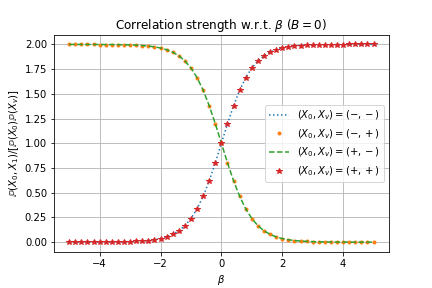
\includegraphics[width=9cm]{img/ising_x0_xv.png}
    \caption{
        We see the correlations for different $\beta$ and $B$ values and $B=0$.
        If and only if $\frac{\pi_{\mu}(x_0, x_v)}{P(x_0)P(x_v)}=1$,
        i.e. $\pi_{\mu}(x_0, x_v) = P(x_0)P(x_v)$ for all $x_0$ and all $x_v$,
        does it mean that $X_0$ and $X_v$ are independent. This only happens at $\beta=0$. The further the values deviate from $1$,
        the more dependence there is. Additionally, We see that as $\beta$ gets
        larger, the $(+, +)$ and $(-, -)$ states are more preferred, and the opposite is true when $\beta$ gets more negative.}
    \label{Fig. x0-xv-correlation}
\end{figure}

$X_0$ and $X_v$ are identically distributed by admissibility. For $B=0$, both $X_0$ and $X_v$ are Bernoulli(1/2). It changes when $B\neq 0$. More
specifically, when $B\rightarrow\infty$, $X_0$ approaches deterministically spin-up. When $B\rightarrow\infty$, $X_0$ approaches deterministically spin-down.
Additionally, the larger $\beta$ is, the faster the switch from spin-down to spin-up is.

\newpage

\begin{figure}[h]
    \centering
    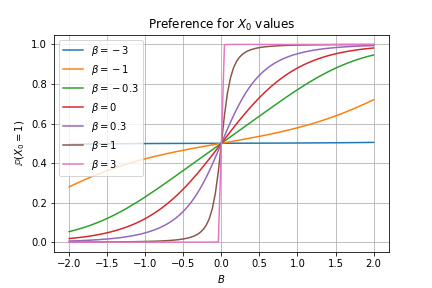
\includegraphics[width=9cm]{img/ising_x0_B.png}
    \caption{$X_0$ prefers $1$ when $B > 0$ and prefers $-1$ when $B < 0$. It is Bernoulli(1/2) when $B=0$. The rate at which $\mathbb{P}(X_0=1)$ increases with $B$ is dependent on $\beta$. The higher the value of $\beta$, the faster it increases.}
    \label{Fig.ising-x0-B}
\end{figure}

For correlation between $X_0$ and $X_v$ when $B\neq 0$. We see that as $|B|$
increases, the negative correlation for $\beta<0$ still goes to $X_0=-X_v$.
However, as $\beta\rightarrow\infty$, we no longer approach $X_0=X_v$. The larger
$|B|$ is, the weaker the correlation between $X_0$ and $X_v$ are at
$\beta\rightarrow\infty$.

\begin{figure}[h]
    \centering
    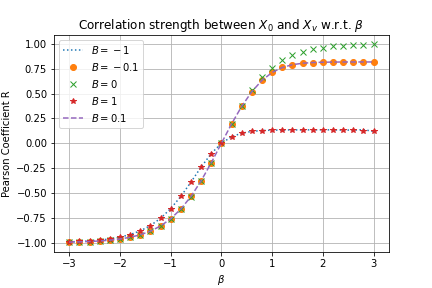
\includegraphics[width=9cm]{img/ising_x0_xv_pearson.png}
    \caption{Correlation strength at $\beta\rightarrow\infty$ for $B\neq 0$ reduces
        as $|B|$ increases. The Pearson coefficient $R=\text{Cov}(X_0, X_v)/\sqrt{\text{Var}(X_0)\text{Var}(X_v)}$ is used to capture the strength of the correlation. Since $X_0$ and $X_v$ are Bernoulli, $R=0$ iff. $X_0, X_v$ independent. We see that $X_0, X_v$ independent iff. $\beta=0$.}
    \label{Fig. ising_x0_xv_B}
\end{figure}

We think that this is due to $B$ strongly biasing to one of the spin-up or spin-down
states, especially at high $\beta$ values. Since $X_0$ and $X_v$ are identically distributed, this results in the highest probability concentrated in one of the states. Pearson coefficient measures the strength of linear correlation, which, when
there is only one state, becomes less accurate.

Since our results are numerical,
and Pearson coefficient depends on the accuracy of small probability, we think that
the trend need to be investigated more to get more conclusive results. The above theory
also does not explain the asymmetry between $\beta\rightarrow\infty$ and $\beta\rightarrow-\infty$.

\subsubsection{Investigating $\mathbb{P}_{\mu^*}(X_1, X_2)$}

For $B=0$, a similar pattern can be observed with $X_1$ and $X_2$. However, this time, as
$|\beta|\rightarrow\infty$, it approaches $X_1=X_2$ no matter if $\beta$ is positive or
negative.

\begin{figure}[h]
    \centering
    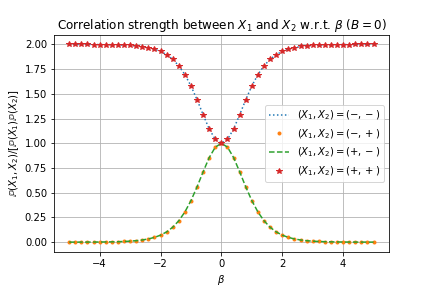
\includegraphics[width=9cm]{./img/ising_x1_x2.png}
    \caption{
        When $B=0$, Similar to $X_0$ and $X_v$, when $\beta=0$, $X_1$ and $X_2$ are independent.
        When $\beta\neq 0$, they become correlated. Their correlation becomes stronger
        as $|\beta|\rightarrow\infty$, and it approaches $X_1=X_2$. Notice that $X_1$ and $X_2$
        are positively correlated in both $\beta > 0$ and $\beta < 0$.}
    \label{Fig.ising-x1-x2}
\end{figure}

For $B\neq 0$, $X_1$ and $X_2$ are still positively-correlated. When $\beta\rightarrow-\infty$, they still approach $X_1=X_2$. However, when
$|B|$ increases, the correlation of $X_1$ and $X_2$ at $\beta\rightarrow\infty$
becomes weaker, similar to the case between $X_0$ and $X_v$.
\begin{figure}[h]
    \centering
    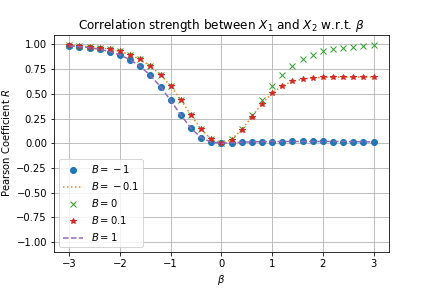
\includegraphics[width=10cm]{img/ising_x1_x2_pearson.png}
    \caption{We see that for $B\neq 0$, the correlation is always a positive correlation, with independence happening iff $\beta=0$.}
    \label{Fig.ising-x1-x2-B}
\end{figure}

\subsubsection{Investigating $\mathbb{P}_{\mu^*}(X_1, X_2|X_0)$}

Given $X_0$, $X_1$ and $X_2$ are always conditionally independent

\begin{figure}[h]
    \centering
    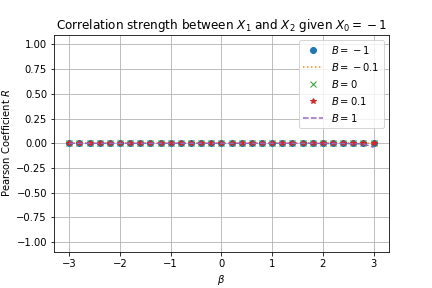
\includegraphics[width=7cm]{img/ising_x1_x2_pearson_x0=-1.png}
    \quad
    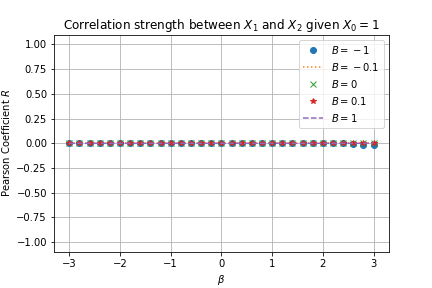
\includegraphics[width=7cm]{img/ising_x1_x2_pearson_x0=1.png}
    \caption{The conditional distributions $X_1|X_0$ and $X_2|X_0$ are always independent}
    \label{Fig.ising-x1-x2-given-x0-B}
\end{figure}

given  suggests a numerical solution in the form
\begin{equation*}
    \mu(x_0,x_1,x_2) = \mu_v(x_1|x_0)\mu_v(x_2|x_0)\mu_0(x_0)
\end{equation*}

\subsection{Partial Analytical solution}

If we assume that $X_0$ and all $X_v$ are identically distributed (given by the admissibility constraint), and that $X_v$ are mutually conditionally independent from each other given $X_0$, we can see that
a distribution can be completely described by two parameters. (This is not
really what the question is asking, but the best I can come up
with.)

First, the probability distribution for $X_0$:
\begin{equation*}
    \mu_0(x):=\mathbb{P}_\mu(X_0=x)
\end{equation*}
This only needs one parameter, as $\mu_0(-)=1-\mu_0(+)$.

Secondly, we need the conditional distribution $X_v|X_0$:
\begin{equation*}
    \nu_\mu(x_0, x) := \mathbb{P}_\mu(X_v=x | X_0=x_0) = \frac{\pi_\mu(x_0, x_v)}{\mu_0(x_0)}
\end{equation*}
This describes $\pi_\mu$. Say $\nu_\mu^- := \nu_\mu(+, -)$, by admissibility,
\begin{align*}
    \pi_\mu(+, +) & = (1-\nu_\mu^-)\mu_0(+)   \\
    \pi_\mu(+, -) & = \nu_\mu^-\mu_0(+)       \\
    \pi_\mu(-, +) & = \nu_\mu^-\mu_0(+)       \\
    \pi_\mu(-, -) & = 1-(1+\nu_\mu^-)\mu_0(+)
\end{align*}
We can then write $\mu$ as a conditional binomial distribution:
\begin{align*}
    \mu(x_0, k) & := \mathbb{P}_\mu\left(X_0=x_0, \sum_{v=1}^\kappa X_v = k\right).                                              \\
    \intertext{Writing as conditional and letting $K:=\sum_{v=1}^\kappa X_v$,}
                & = \mathbb{P}_\mu(X_0=x_0)\mathbb{P}_\mu\left(K=k | X_0=x_0\right)                                              \\
                & = \mu_0(x_0) {\kappa\choose k}\mathbb{P}_\mu(X_v=+ | X_0=x_0)^k(1-\mathbb{P}_\mu(X_v=+ | X_0=x_0))^{\kappa-k}.
\end{align*}
Hence,
\begin{align*}
    \mu(+, k) & = \mu_0(+){\kappa\choose k}\left(1-\nu_\mu^-\right)^k\left(\nu_\mu^-\right)^{\kappa-k}                                                                \\
    \mu(-, k) & = [1-\mu_0(+)]{\kappa\choose k}\left[\frac{\nu_\mu^-\mu_0(+)}{1-\mu_0(+)}\right]^k\left[\frac{1-(1+\nu_\mu^-)\mu_0(+)}{1-\mu_0(+)}\right]^{\kappa-k}.
\end{align*}
Optimizing with respect to $\mu_0(+)$ and $\nu_\mu^-$ should give the desired results.

\newpage

\section{Jun 19 - Jun 24}

\subsection{Numerical Solution to Edward-Anderson}

\subsubsection{Formulation}

For each of the $\kappa$ vertices, there are 4 possible states for $(y_{0v}, x_v)$: $(-, -), (-, +), (+, -), (+, +)$.
They are labelled by an index in ascending order (0 through 3).

To label each state that the tree can take, we describe it as $(x_0, k_0, k_1, k_2, k_3)$, where $x_0$ is the spin-state of the root vertex,
and $k_\ell$ is the number of vertices in the edge-vertex state of $\ell$ ($\ell=0:3$). Since we have $\kappa$ vertices in total, $\kappa=k_0+k_1+k_2+k_3$.
More compactly, we can enumerate each distinct choice of $(k_0, k_1, k_2, k_3)$ that sums to $\kappa$ with an index $i$. This will be recorded in
a matrix $C$, where $C_{i\ell}$ is the number of vertices in state $\ell$ for the $i$-th edge-vertex configuration.

The following is an example for $\kappa=2$:

\begin{equation*}
    \begin{bmatrix}
        0 & 0 & 0 & 2 \\
        0 & 0 & 1 & 1 \\
        0 & 0 & 2 & 0 \\
        0 & 1 & 0 & 1 \\
        0 & 1 & 1 & 0 \\
        1 & 0 & 0 & 1 \\
        1 & 0 & 1 & 0 \\
        0 & 2 & 0 & 0 \\
        1 & 1 & 0 & 0 \\
        2 & 0 & 0 & 0
    \end{bmatrix}
\end{equation*}
Note that $i$ can take ${\kappa+3 \choose 3}$ values. This is equivalent to arranging $\kappa$ symbols and $4-1$ separators:
% \begin{figure}[h]
%     \centering
%     
\includegraphics[width=5cm]{img/SCR-20230619-ujrs.png}
%     % \caption{https://tjyusun.com/mat202/sec-balls-in-bins.html#:~:text=of\%20size\%20is-,.,distribute\%20indistinguishable\%20balls\%20into\%20bins.}
% \end{figure}

Hence, for the Hamiltonian,
\begin{align*}
    \mathcal{H}(x_0, i) = \frac\beta2x_0(C_{i0} - C_{i1} - C_{i2} + C_{i3}) + Bx_0
\end{align*}
We represent the distribution as $\mu_{x_0, i}$, where $\sum_{x_0\in \mathcal{X}}\sum_{i=1}^{\kappa+3 \choose 3} \mu_{x_0, i} = 1$.
The distribution on the edge becomes
\begin{align*}
    \pi_\mu(x_0, y_{0v}, x_v) & = \frac1\kappa\mathbb{E}_\mu\left[\sum_{v\in\mathcal{N_0(\tau)}}\mathbf{1}_{\{X_0=x_0, Y_{0v}=y_{0v}, X_v=x_v\}}\right] \\
    \pi_\mu(x_0, \ell)        & = \frac1\kappa\sum_{i=1}^{\kappa+3 \choose 3} C_{i\ell}\mu_{x_0, i}
\end{align*}
where $\ell$ corresponds to $(y_{0v}, x_v)$.

This means that the admissibility constraint
\begin{equation*}
    \pi_\mu(x_0, y_{0v}, x_v) = \pi_\mu(x_v, y_{0v}, x_0) \quad \forall x_0, y_{0v}, x_v
\end{equation*}
reduces to two equalities:
\begin{equation*}
    \begin{cases}
        \pi_\mu(+, -, -) & = \pi_\mu(-, -, +) \\
        \pi_\mu(+, +, -) & = \pi_\mu(-, +, +)
    \end{cases}
    \Rightarrow
    \begin{cases}
        \pi_\mu(+, 0) & = \pi_\mu(-, 1) \\
        \pi_\mu(+, 2) & = \pi_\mu(-, 3)
    \end{cases}
\end{equation*}

Optimizations are performed with initial condition $\eta$ and objective function tolerance $10^{-10}$ with SLSQP in SciPy.

\subsubsection{Conditional independence}

One of the objects of interest is the joint conditional distribution of two distinct edge-vertex pairs given the root:
\begin{equation*}
    \mathbb{P}_\mu\left[(X_v, Y_{0v}) = (x_v, y_{0v}), (X_{v'}, Y_{0v'}) = (x_{v'}, y_{0v'}) | X_0 = x_0\right]
\end{equation*}
Due to the permutation symmetry on the leaf nodes, it is simpler to calculate the joint distribution on all edge-vertex
pairs and take the marginal (This is not necessary for $\kappa=2$). Say
\begin{equation*}
    \nu_\mu[(x_1, y_{01}), \ldots, (x_\kappa, y_{0\kappa})| x_0] = \mathbb{P}_\mu\left[(X_1, Y_{01}) = (x_1, y_{01}), \ldots,  (X_{\kappa}, Y_{0\kappa}) = (x_{\kappa}, y_{0\kappa}) | X_0 = x_0\right]
\end{equation*}
Similar to Ising, to get $\nu_\mu$, we only need to remove multiplicity, this time given by a multinomial coefficient:
\begin{equation*}
    \nu_\mu[(x_1, y_{01}), \ldots, (x_\kappa, y_{0\kappa})| x_0] = \frac{1}{{\kappa \choose {k_0\ k_1\ k_2\ k_3}}\mu_0(x_0)}\mu_{x_0, k_0, k_1, k_2, k_3}
\end{equation*}
where $k_l$ is the number of leaves with edge-vertex $(x_v, y_{0v})$ in state $l$, $\mu_0$ is the marginal distribution on the root with $\mu_0(x_0) = \sum_{i=1}^{{\kappa+3\choose 3}} \mu_{x_0, i}$, and the multinomial coefficient
\begin{equation*}
    {\kappa \choose {k_0\ k_1\ k_2\ k_3}} = \frac{\kappa!}{k_0!k_1!k_2!k_3!}.
\end{equation*}

We hypothesize that vertex-edge marks are conditionally independent given the root mark, i.e.
\begin{equation*}
    \nu_\mu[(x_1, y_{01}), \ldots, (x_\kappa, y_{0\kappa})| x_0] = \prod_{v=1}^\kappa \nu_\mu^{v|0} [(x_v, y_{0v}) | x_0]
\end{equation*}
where $\nu_\mu^{v|0} [(x_v, y_{0v}) | x_0]$ is the marginal conditional distribution.

To compare these two, we name the conditional dependent form $\check{\nu}_\mu = \prod_{v=1}^\kappa \nu_\mu^{v|0}$. We want to prove that $\nu_\mu = \check{\nu}_\mu$. We will compare them with relative entropy $H(\nu_\mu \| \check{\nu}_\mu)$. $\nu_\mu = \check{\nu}_\mu$ if and only if $H(\nu_\mu \| \check{\nu}_\mu) = 0$.

\newpage

Indeed, numerically, $H(\nu_\mu \| \check{\nu}_\mu)$ is close to $0$ for all $\beta$ and $B$.
\begin{figure}[h]
    \centering
    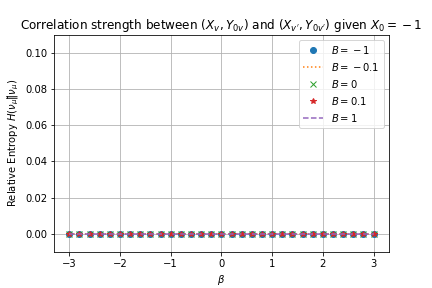
\includegraphics[width=7.5cm]{img/EA_x1_x2_RelEntr_x0=-1.png}
    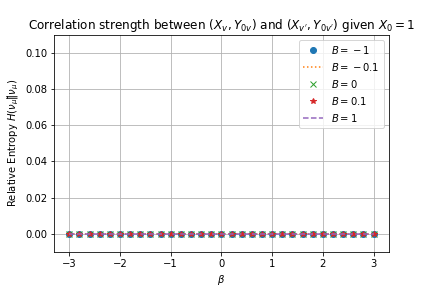
\includegraphics[width=7.5cm]{img/EA_x1_x2_RelEntr_x0=1.png}
    \caption{For Edward-Anderson model $\kappa=2$, the conditional joint distribution of edge-vertex marks given the root marks $\nu_\mu$
        has a zero distance w.r.t. the conditional independent form $\check{\nu}_\mu$. This is confirmed with different values of $\beta$ and $B$.}
    \label{Fig.EA-x1-x2-given-x0-rel-entr}
\end{figure}

\subsubsection{Root mark distribution with respect to external field}

\begin{figure}[h]
    \centering
    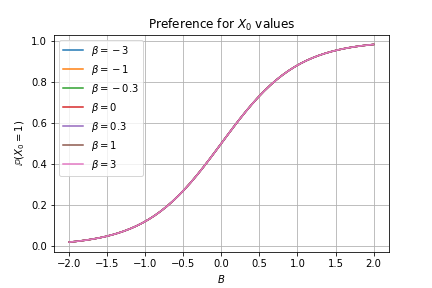
\includegraphics[width=12cm]{img/EA_x0_B.png}
    \caption{For Edward-Anderson model $\kappa=2$, the distribution of the root mark is only dependent on $B$, and not dependent on $\beta$. }
    \label{Fig.EA-x0-B}
\end{figure}

Getting the marginal distribution on the root, write the distribution in the form
\begin{equation*}
    \mu_0(x_0) = \frac1Z\exp[f(\beta, B)x_0]
\end{equation*}
where $f(\beta, B)$ is some function of the parameters.

Therefore, to extract the information, we have that
\begin{equation*}
    \log \frac{\mu_0(+)}{1 - \mu_0(+)} = 2f(\beta, B).
\end{equation*}
In fact, assuming that the distribution is not dependent on $\beta$, $f$ should not be dependent on $\beta$.
\begin{figure}[h]
    \centering
    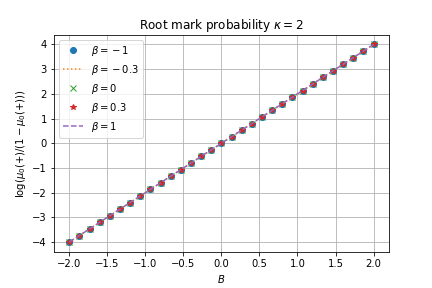
\includegraphics[width=12cm]{img/EA_x0_B_logisitic_kappa_2.png}
    \caption{For Edward-Anderson model $\kappa=2$, we see that $2f(\beta, B) = 2B$, thus giving a distribution in the form $\mu_0(x_0) = \frac{e^{Bx_0}}{e^B + e^{-B}}$. }
    \label{Fig.EA-x0-B-logisitic}
\end{figure}

If we increase $\kappa$, we see similar results, but with slightly higher uncertainty (Fig.\ref{Fig.EA-x0-B-logisitic-change-kappa}).
zero
\begin{figure}[h]
    \centering
    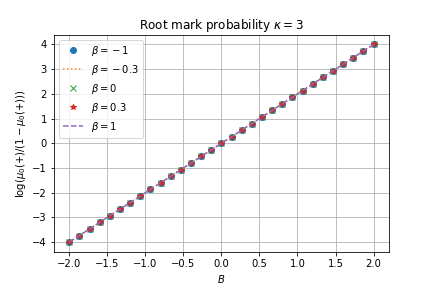
\includegraphics[width=7.5cm]{img/EA_x0_B_logisitic_kappa_3.png}
    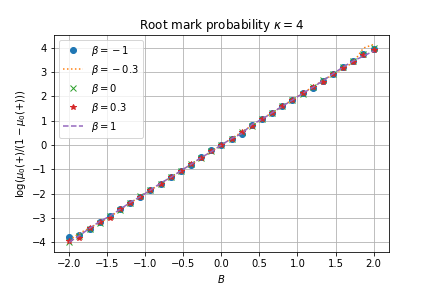
\includegraphics[width=7.5cm]{img/EA_x0_B_logisitic_kappa_4.png}
    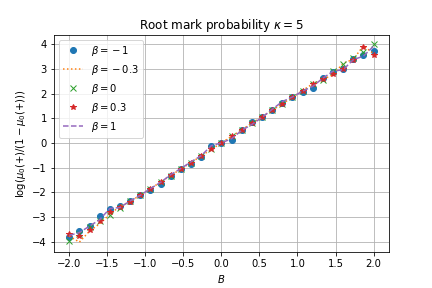
\includegraphics[width=7.5cm]{img/EA_x0_B_logisitic_kappa_5.png}
    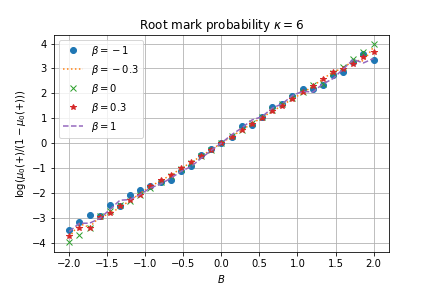
\includegraphics[width=7.5cm]{img/EA_x0_B_logisitic_kappa_6.png}
    \caption{For Edward-Anderson model with $\kappa=3, 4, 5, 6$, we see that the root mark distribution is roughly the same. }
    \label{Fig.EA-x0-B-logisitic-change-kappa}
\end{figure}
\newpage
Since we cannot impose tolerance on the optimized vector, we see that the optimization algorithm struggles to get the ones with
higher $\kappa$ values and higher $|B|$ values. Higher $B$ values tend to cause multiscale values in the distribution $\mu$, i.e.
some values in $\mu$ are orders of magnitude larger than others. For example, for $\kappa=6$, $B=2$, we have values as large as $0.396$
and as small as $2.43e-12$. This, combined with the much higher dimensionality of $\mu$ ($\mathbb{R}^{168}$ for
$\kappa=2$) may have contributed to the higher uncertainties. However, the prediction is likely still consistent with $f(\beta, B) = B$.

\newpage
\subsection{Analytical solution to Ising}

For $\mu$, we switch to a different convention, where $\mu(x_0, k)$ represents the probability that root vertex is in $x_0$ and there are
$k$ leaf nodes in the same spin as the root vertex.
We can rewrite the Hamiltonian:
\begin{equation*}
    \mathcal{H}(x_0, k) = \frac\beta2(2k-\kappa) + Bx_0
\end{equation*}
Assuming that the distribution $\mu$ has leaf vertex that are conditionally independent on the root vertex, we can write the distribution as
\begin{equation*}
    \mu(x_0, k) = \mu_0(x_0){\kappa \choose k}\left[\pi_\mu^{v|0}(x_0|x_0)\right]^k\left[\pi_\mu^{v|0}(-x_0|x_0)\right]^{\kappa - k}
\end{equation*}
where $\mu_0(x_0)=\sum_{k=0}^\kappa \mu(x_0, k)$ is the marginal distribution on the root vertex, and
$\pi_\mu^{v|0}(x_v|x_0) = \pi_\mu(x_0, x_v) / \mu_0(x_0)$ is the conditional distribution on one of the leaf vertices.

Define $\mu_0^+ = \mu_0(+)$, $\mu_0^- = \mu_0(+)$, $\gamma_\mu^+=\pi_\mu^{v|0}(+|+)$, $\gamma_\mu^-=\pi_\mu^{v|0}(-|-)$. We have
\begin{equation*}
    \begin{aligned}
        \mu_0^+ & = \sum_{k=0}^\kappa \mu(+, k) \\
        \mu_0^- & = \sum_{k=0}^\kappa \mu(-, k)
    \end{aligned}
    \quad\quad\quad
    \begin{aligned}
        \gamma_\mu^+ & = \frac{1}{\kappa\mu_0^+} \sum_{k=0}^\kappa k \mu(+, k) \\
        \gamma_\mu^- & = \frac{1}{\kappa\mu_0^-} \sum_{k=0}^\kappa k \mu(-, k)
    \end{aligned}
\end{equation*}
and
\begin{align*}
    \mu(+, k) = \mu_0^+{\kappa \choose k}\left(\gamma_\mu^+\right)^k\left(1 - \gamma_\mu^+\right)^{\kappa - k} \\
    \mu(-, k) = \mu_0^-{\kappa \choose k}\left(\gamma_\mu^-\right)^k\left(1 - \gamma_\mu^-\right)^{\kappa - k}
\end{align*}
For the distribution to be normalized, $\mu_0^++\mu_0^-=1$, and the symmetry constraint is
\begin{equation*}
    \mu_0^+(1-\gamma_\mu^+) = \mu_0^-(1-\gamma_\mu^-)
\end{equation*}

The objective function (using I-Hsun's convention) is
\begin{equation*}
    V = \mathbb{E}_\mu \mathcal{H}(X_0, \tau) - \left\{H(\mu_0\|\eta_0) + \frac12\left[H(\mu\|\check{\mu}) + H(\mu\|\hat{\mu})\right]\right\}
\end{equation*}
Simplifying each term:
\begin{align*}
      & \mathbb{E}_\mu \mathcal{H}(X_0, \tau)                                                       \\
    = & \sum_{k=0}^\kappa \mu(+, k)\mathcal{H}(+, k) + \sum_{k=0}^\kappa \mu(-, k)\mathcal{H}(-, k) \\
    = & \sum_{k=0}^\kappa \mu(+, k)\left[\frac\beta2 (2k-\kappa) + B\right] +
    \sum_{k=0}^\kappa \mu(-, k)\left[\frac\beta2 (2k-\kappa) - B\right]                             \\
    = & \beta \left[\sum_{k=0}^\kappa k\mu(+, k) + \sum_{k=0}^\kappa k\mu(-, k) \right] -
    \frac\beta2 \kappa\left[\sum_{k=0}^\kappa \mu(+, k) + \sum_{k=0}^\kappa \mu(-, k)\right] +
    B\left[\sum_{k=0}^\kappa \mu(+, k) - \sum_{k=0}^\kappa \mu(-, k)\right]                         \\
    = & \beta \kappa\left(\mu_0^+\gamma_\pi^+ + \mu_0^-\gamma_\pi^-\right)
    + B\left(\mu_0^+ - \mu_0^-\right) - \frac{\beta\kappa}{2}
\end{align*}
Continuing,
\begin{align*}
    H(\mu_0\|\eta_0) = \mu_0^+\log\frac{\mu_0^+}{\eta_0^+} + \mu_0^-\log\frac{\mu_0^-}{\eta_0^-}
\end{align*}
And since $\mu$ is assumed to be conditionally independent on $X_0$, we know that $H(\mu\|\hat{\mu}) = 0$.

On the other hand,
\begin{align*}
      & H(\mu \| \check{\mu})                                                                                   \\
    = & \sum_{k=0}^\kappa \mu(+, k)\log\frac{\mu(+, k)}{\check{\mu}(+, k)}
    + \sum_{k=0}^\kappa \mu(-, k)\log\frac{\mu(-, k)}{\check{\mu}(-, k)}                                        \\
    = & \sum_{k=0}^\kappa \mu(+, k)\log\frac{
    \mu_0^+{\kappa \choose k}\left(\gamma_\mu^+\right)^k\left(1 - \gamma_\mu^+\right)^{\kappa - k}
    }{
    \mu_0^+{\kappa \choose k}\left(\mu_0^+\right)^k\left(\mu_0^-\right)^{\kappa - k}}
    + \sum_{k=0}^\kappa \mu(-, k)\log\frac{
    \mu_0^-{\kappa \choose k}\left(\gamma_\mu^-\right)^k\left(1 - \gamma_\mu^-\right)^{\kappa - k}
    }{
    \mu_0^-{\kappa \choose k}\left(\mu_0^-\right)^k\left(\mu_0^+\right)^{\kappa - k}}                           \\
    = & \sum_{k=0}^\kappa \mu(+, k)\log\frac{
        \left(\gamma_\mu^+\right)^k\left(1 - \gamma_\mu^+\right)^{\kappa - k}
    }{
        \left(\mu_0^+\right)^k\left(\mu_0^-\right)^{\kappa - k}}
    + \sum_{k=0}^\kappa \mu(-, k)\log\frac{
        \left(\gamma_\mu^-\right)^k\left(1 - \gamma_\mu^-\right)^{\kappa - k}
    }{
    \left(\mu_0^-\right)^k\left(\mu_0^+\right)^{\kappa - k}}                                                    \\
    = & \sum_{k=0}^\kappa \mu(+, k)\left[\log\frac{
            \left(\gamma_\mu^+\right)^k\left(1 - \gamma_\mu^+\right)^{-k}
        }{
            \left(\mu_0^+\right)^k\left(\mu_0^-\right)^{-k}}
    + \log \frac{\left(1 - \gamma_\mu^+\right)^\kappa}{\left(\mu_0^-\right)^\kappa}\right]                      \\
      & + \sum_{k=0}^\kappa \mu(-, k)\left[\log\frac{
            \left(\gamma_\mu^-\right)^k\left(1 - \gamma_\mu^-\right)^{-k}
        }{
            \left(\mu_0^-\right)^k\left(\mu_0^+\right)^{-k}}
    + \log\frac{\left(1 - \gamma_\mu^-\right)^\kappa}{\left(\mu_0^+\right)^\kappa}\right]                       \\
    = & \sum_{k=0}^\kappa \mu(+, k)\left[k\log\frac{\gamma_\mu^+ \mu_0^-}{\mu_0^+\left(1 - \gamma_\mu^+\right)}
        + \kappa\log\frac{1 - \gamma_\mu^+}{\mu_0^-}\right]
    + \sum_{k=0}^\kappa \mu(-, k)\left[k\log\frac{\gamma_\mu^- \mu_0^+}{\mu_0^-\left(1 - \gamma_\mu^-\right)}
    + \kappa\log\frac{1 - \gamma_\mu^-}{\mu_0^+}\right]                                                         \\
    = & \kappa\mu_0^+\gamma_\mu^+\log\frac{\gamma_\mu^+ \mu_0^-}{\mu_0^+\left(1 - \gamma_\mu^+\right)}
    + \kappa\mu_0^+\log\frac{1 - \gamma_\mu^+}{\mu_0^-}
    + \kappa\mu_0^-\gamma_\mu^-\log\frac{\gamma_\mu^- \mu_0^+}{\mu_0^-\left(1 - \gamma_\mu^-\right)}
    + \kappa\mu_0^-\log\frac{1 - \gamma_\mu^-}{\mu_0^+}
    \intertext{According to the symmetry constraint, $\mu_0^+(1-\gamma_\mu^+) = \mu_0^-(1-\gamma_\mu^-)$, so}
    = & \kappa\mu_0^+\gamma_\mu^+\log\frac{\gamma_\mu^+ \mu_0^-}{\mu_0^-\left(1 - \gamma_\mu^-\right)}
    + \kappa\mu_0^+\log\frac{1 - \gamma_\mu^+}{\mu_0^-}
    + \kappa\mu_0^-\gamma_\mu^-\log\frac{\gamma_\mu^- \mu_0^+}{\mu_0^+\left(1 - \gamma_\mu^+\right)}
    + \kappa\mu_0^-\log\frac{1 - \gamma_\mu^-}{\mu_0^+}                                                         \\
    = & \kappa\mu_0^+\gamma_\mu^+\log\frac{\gamma_\mu^+}{1 - \gamma_\mu^-}
    + \kappa\mu_0^+\log\frac{1 - \gamma_\mu^+}{\mu_0^-}
    + \kappa\mu_0^-\gamma_\mu^-\log\frac{\gamma_\mu^-}{1 - \gamma_\mu^+}
    + \kappa\mu_0^-\log\frac{1 - \gamma_\mu^-}{\mu_0^+}                                                         \\
\end{align*}

\newpage
We can rewrite the objective function:
\begin{align*}
    V = & \beta \kappa\left(\mu_0^+\gamma_\pi^+ + \mu_0^-\gamma_\pi^-\right)
    + B\left(\mu_0^+ - \mu_0^-\right)
    - \mu_0^+\log\frac{\mu_0^+}{\eta_0^+} - \mu_0^-\log\frac{\mu_0^-}{\eta_0^-}      \\
        & - \frac\kappa2\mu_0^+\gamma_\mu^+\log\frac{\gamma_\mu^+}{1 - \gamma_\mu^-}
    - \frac\kappa2\mu_0^+\log\frac{1 - \gamma_\mu^+}{\mu_0^-}
    - \frac\kappa2\mu_0^-\gamma_\mu^-\log\frac{\gamma_\mu^-}{1 - \gamma_\mu^+}
    - \frac\kappa2\mu_0^-\log\frac{1 - \gamma_\mu^-}{\mu_0^+}
\end{align*}
and the corresponding Lagrangian is
\begin{equation*}
    \tilde{V} = V + \lambda(\mu_0^+(1-\gamma_\mu^+) - \mu_0^-(1-\gamma_\mu^-)) + \gamma (\mu_0^+ + \mu_0^- - 1)
\end{equation*}
Solving for $\gamma_\mu^+$:
\begin{align*}
    \partial_{\gamma_\mu^+} \tilde{V} = \beta\kappa\mu_0^+ -\frac\kappa2\mu_0^+\left(\log\frac{\gamma_\mu^+}{1-\gamma_\mu^-} + 1\right)
    + \frac\kappa2\frac{\mu_0^+}{1-\gamma_\mu^+} - \frac\kappa2\mu_0^-\gamma_\mu^-\frac{1}{1-\gamma_\mu^+}-\lambda\mu_0^+ & = 0 \\
    2\beta - \left(\log\frac{\gamma_\mu^+}{1-\gamma_\mu^-} + 1\right)
    + \frac{1}{1-\gamma_\mu^+} - \frac{\mu_0^-}{\mu_0^+}\frac{\gamma_\mu^-}{1-\gamma_\mu^+}-\frac{2\lambda}{\kappa}       & = 0 \\
    \intertext{by the symmetry constraint, }
    2\beta - \left(\log\frac{\gamma_\mu^+}{1-\gamma_\mu^-} + 1\right)
    + \frac{1}{1-\gamma_\mu^+} - \frac{\mu_0^-}{\mu_0^-}\frac{\gamma_\mu^-}{1-\gamma_\mu^-}-\frac{2\lambda}{\kappa}       & = 0 \\
    2\beta - \left(\log\frac{\gamma_\mu^+}{1-\gamma_\mu^-} + 1\right)
    + \frac{1}{1-\gamma_\mu^+} - \frac{\gamma_\mu^-}{1-\gamma_\mu^-}-\frac{2\lambda}{\kappa}                              & = 0
\end{align*}
Similarly,
\begin{equation*}
    2\beta - \left(\log\frac{\gamma_\mu^-}{1-\gamma_\mu^+} + 1\right)
    + \frac{1}{1-\gamma_\mu^-} - \frac{\gamma_\mu^+}{1-\gamma_\mu^+}+\frac{2\lambda}{\kappa}= 0
\end{equation*}
We should be able to solve for $\gamma_\mu^+$ and $\gamma_\mu^-$ with these two equations.

\newpage

\section{Jun 25 - 30}

\subsection{Edward-Anderson (Reduced) Analytical}

For the Edward-Anderson Model, as discussed above, we model the edge-vertex configurations with counts $(k_{y, x})_{y\in\mathcal{Y}, x\in\mathcal{X}}$, where $k_{y, x}$ counts the number of edge-vertex pairs that have edge-mark of $y$ and vertex mark of $x$. This has an added constraint that
\begin{equation}
    \sum_{y\in\mathcal{Y}}\sum_{x\in\mathcal{X}} k_{y, x} = \kappa
\end{equation}
we can define a vector $\mathbf{k}\in \mathcal{K}$ such that $\mathcal{K} = \{(k_{y, x})_{y\in\mathcal{Y}, x\in\mathcal{X}} : \sum_{y\in\mathcal{Y}}\sum_{x\in\mathcal{X}} k_{y, x} = \kappa\}$ to represent the full state.

In the case that $\mathcal{Y} = \{-1, 1\}$, we can rewrite
\begin{equation}
    \mathcal{H}(x_0, \mathbf{k}) = \frac\beta2 x_0 (k_{++} - k_{+-} - k_{-+} + k_{--}) + Bx_0 \quad\forall \mathbf{k}\in\mathbb{K}
\end{equation}
And $\eta$ is:
\begin{equation*}
    \eta(x_0, \mathbf{k}) = {\kappa \choose \mathbf{k}} 2^{-(2\kappa+1)} \quad\forall \mathbf{k}\in\mathbb{K}
\end{equation*}
where ${\kappa \choose \mathbf{k}} = {\kappa \choose k_{++}\ k_{+-}\ k_{-+}\ k_{--}} = \frac{\kappa!}{k_{++}!k_{+-}!k_{-+}!k_{--}!}$ is the
multinomial coefficient.

Additionally, the edge distribution becomes
\begin{equation}
    \pi_\mu(x_0, y_{0v}, x_v) = \frac1\kappa \sum_{\mathbf{k}\in \mathcal{K}} k_{y_{0v}, x_v} \mu(x_0, \mathbf{k})
\end{equation}
Our objective function is
\begin{equation}
    V(\beta, B, \kappa, \mu) = \mathbb{E}_\mu \mathcal{H}(\tau, X, Y) - H(\mu \| \eta) + \frac\kappa2 H(\pi_\mu \| \pi_\eta)
\end{equation}
Rewriting each term:
\begin{align*}
    \mathbb{E}_\mu \mathcal{H}(\tau, X, Y)                                                                                                  = & \sum_{\mathbf{k}\in\mathcal{K}}[\mu(+, \mathbf{k}) - \mu(-, \mathbf{k})]\left[\frac\beta2(k_{++} - k_{+-} - k_{-+} + k_{--}) + B\right]                                                                                                                                             \\
    =                                                                                                                                         & \sum_{x_0\in\mathcal{X}}\sum_{y_{0v}\in\mathcal{Y}}\sum_{x_v\in\mathcal{X}}x_0 y_{0v} x_v\sum_{\mathbf{k}\in\mathcal{K}} k_{y_{0v}, x_v} \mu(x_0, \mathbf{k}) + B\left[\sum_{\mathbf{k}\in\mathcal{K}}\mu(+, \mathbf{k}) - \sum_{\mathbf{k}\in\mathcal{K}}\mu(-, \mathbf{k})\right]
\end{align*}
and for the relative entropy terms:
\begin{align*}
    H(\mu \| \eta) & = \sum_{x_0\in\mathcal{X}}\sum_{\mathbf{k}\in\mathcal{K}}\mu(x_0, \mathbf{k})\log\mu(x_0, \mathbf{k})
    - \sum_{x_0\in\mathcal{X}}\sum_{\mathbf{k}\in\mathcal{K}}\mu(x_0, \mathbf{k})\log\eta(x_0, \mathbf{k})                 \\
                   & = \sum_{x_0\in\mathcal{X}}\sum_{\mathbf{k}\in\mathcal{K}}\mu(x_0, \mathbf{k})\log\mu(x_0, \mathbf{k})
    - \sum_{x_0\in\mathcal{X}}\sum_{\mathbf{k}\in\mathcal{K}}\mu(x_0, \mathbf{k})\log{\kappa \choose \mathbf{k}}
    + (2\kappa + 1)\log 2
\end{align*}
and
\begin{align*}
      & H(\pi_\mu \| \pi_\eta)                                                                                \\
    = & \sum_{x_0\in\mathcal{X}}\sum_{y_{0v}\in\mathcal{Y}}\sum_{x_v\in\mathcal{X}}
    \pi_\mu(x_0, y_{0v}, x_v)\log \pi_\mu(x_0, y_{0v}, x_v) -
    \sum_{x_0\in\mathcal{X}}\sum_{y_{0v}\in\mathcal{Y}}\sum_{x_v\in\mathcal{X}}
    \pi_\mu(x_0, y_{0v}, x_v)\log \pi_\eta(x_0, y_{0v}, x_v)                                                  \\
    = & \sum_{x_0\in\mathcal{X}}\sum_{y_{0v}\in\mathcal{Y}}\sum_{x_v\in\mathcal{X}}
    \left[\frac1\kappa\sum_{\mathbf{k}\in\mathcal{K}}k_{y_{0v}, x_v}\mu(x_0, \mathbf{k})\right]
    \log \left[\frac1\kappa\sum_{\mathbf{k}\in\mathcal{K}}k_{y_{0v}, x_v}\mu(x_0, \mathbf{k})\right] + \log 8 \\
    = & \frac1\kappa\sum_{x_0\in\mathcal{X}}\sum_{y_{0v}\in\mathcal{Y}}\sum_{x_v\in\mathcal{X}}
    \left[\sum_{\mathbf{k}\in\mathcal{K}}k_{y_{0v}, x_v}\mu(x_0, \mathbf{k})\right]
    \log \left[\sum_{\mathbf{k}\in\mathcal{K}}k_{y_{0v}, x_v}\mu(x_0, \mathbf{k})\right] + \log \frac8\kappa
\end{align*}
Hence, the objective function becomes
\begin{equation}
    \begin{aligned}
          & V(\beta, B, \kappa, \mu)                                                                                                                                                                                                                                                            \\
        = & \sum_{x_0\in\mathcal{X}}\sum_{y_{0v}\in\mathcal{Y}}\sum_{x_v\in\mathcal{X}}x_0 y_{0v} x_v\sum_{\mathbf{k}\in\mathcal{K}} k_{y_{0v}, x_v} \mu(x_0, \mathbf{k}) + B\left[\sum_{\mathbf{k}\in\mathcal{K}}\mu(+, \mathbf{k}) - \sum_{\mathbf{k}\in\mathcal{K}}\mu(-, \mathbf{k})\right] \\
          & - \sum_{x_0\in\mathcal{X}}\sum_{\mathbf{k}\in\mathcal{K}}\mu(x_0, \mathbf{k})\log\mu(x_0, \mathbf{k})
        + \sum_{x_0\in\mathcal{X}}\sum_{\mathbf{k}\in\mathcal{K}}\mu(x_0, \mathbf{k})\log{\kappa \choose \mathbf{k}}                                                                                                                                                                            \\
          & + \frac12\sum_{x_0\in\mathcal{X}}\sum_{y_{0v}\in\mathcal{Y}}\sum_{x_v\in\mathcal{X}}
        \left[\sum_{\mathbf{k}\in\mathcal{K}}k_{y_{0v}, x_v}\mu(x_0, \mathbf{k})\right]
        \log \left[\sum_{\mathbf{k}\in\mathcal{K}}k_{y_{0v}, x_v}\mu(x_0, \mathbf{k})\right]                                                                                                                                                                                                    \\
          & - (2\kappa + 1)\log 2 + \frac\kappa2 \log \frac8\kappa
    \end{aligned}
    \label{Eq.Objective-expanded}
\end{equation}
Similar to I-Hsun's notes, we notice that besides line 2 of (\ref{Eq.Objective-expanded}):
\begin{equation}
    - \sum_{x_0\in\mathcal{X}}\sum_{\mathbf{k}\in\mathcal{K}}\mu(x_0, \mathbf{k})\log\mu(x_0, \mathbf{k})
    + \sum_{x_0\in\mathcal{X}}\sum_{\mathbf{k}\in\mathcal{K}}\mu(x_0, \mathbf{k})\log{\kappa \choose \mathbf{k}}
    \label{Eq.EA-intermediate-obj}
\end{equation}
everything else is dependent on $\sum_{\mathbf{k}\in\mathcal{K}} k_{y_{0v}, x_v}\mu(x_0, \mathbf{k})$ and
$\sum_{\mathbf{k}\in\mathcal{K}}\mu(x_0, \mathbf{k})$, the latter a linear combination of the former. We optimize for $\mu$
subject to the constraints: $\sum_{\mathbf{k}\in\mathcal{K}} k_{y_{0v}, x_v}\mu(x_0, \mathbf{k}) = m^{x_0, y_{0v}, x_v}$,
$\sum_{\mathbf{k}\in\mathcal{K}}\mu(+, \mathbf{k}) + \sum_{\mathbf{k}\in\mathcal{K}}\mu(-, \mathbf{k}) = 1$, and
$\sum_{\mathbf{k}\in\mathcal{K}}\mu(+, \mathbf{k}) - \sum_{\mathbf{k}\in\mathcal{K}}\mu(-, \mathbf{k}) = m$.

Solving the problem gives the following solution:
\begin{equation}
    \begin{cases}
        \mu(+, \mathbf{k}) = \displaystyle{\frac{e^\gamma}{Z}{\kappa\choose\mathbf{k}} \prod_{y_\in\mathcal{Y}, x\in\mathcal{X}}\left(q^{+,y,x}\right)^{k_{y,x}}}    \\
        \mu(-, \mathbf{k}) = \displaystyle{\frac{e^{-\gamma}}{Z}{\kappa\choose\mathbf{k}} \prod_{y_\in\mathcal{Y}, x\in\mathcal{X}}\left(q^{-,y,x}\right)^{k_{y,x}}} \\
    \end{cases}
    \label{Eq.dist-form1}
\end{equation}
where $Z = e^\gamma\left(\sum_{y_\in\mathcal{Y}, x\in\mathcal{X}}q^{+,y,x}\right)^\kappa + e^{-\gamma}\left(\sum_{y_\in\mathcal{Y}, x\in\mathcal{X}}q^{-,y,x}\right)^\kappa$ is the normalizing constant.

For the distribution to be symmetric, we need
\begin{align}
    \pi_\mu(+, +, -) = \pi_\mu(-, +, +) \label{Eq.EA-reduced-Sym-constr1} \\
    \pi_\mu(+, -, -) = \pi_\mu(-, -, +) \label{Eq.EA-reduced-Sym-constr2}
\end{align}
Substituting (\ref{Eq.dist-form1}) into (\ref{Eq.EA-reduced-Sym-constr1}), we have
\begin{align}
    \sum_{k\in\mathcal{K}}k_{+-}\mu(+, \mathbf{k})                                                       & = \sum_{k\in\mathcal{K}}k_{++}\mu(-, \mathbf{k})                                                         \nonumber                       \\
    e^\gamma\kappa q^{++-} \left(\sum_{{y_\in\mathcal{Y}, x\in\mathcal{X}}}q^{+, y, x}\right)^{\kappa-1} & = e^{-\gamma}\kappa q^{-++} \left(\sum_{{y_\in\mathcal{Y}, x\in\mathcal{X}}}q^{-, y, x}\right)^{\kappa-1} \label{Eq.EA-reduced-Sym-soln}
\end{align}
Using (\ref{Eq.EA-reduced-Sym-soln}) in (\ref{Eq.dist-form1}) gives
\begin{equation}
    \begin{cases}
        \mu(+, \mathbf{k}) = \displaystyle{\frac{q^{-++}\sum_{y, x}q^{+,y,x}}{q^{-++}\sum_{y, x}q^{+,y,x} + q^{++-}\sum_{y, x}q^{-,y,x}}{\kappa\choose\mathbf{k}} \prod_{y_\in\mathcal{Y}, x\in\mathcal{X}}\left(\frac{q^{+,y,x}}{\sum_{y', x'}q^{+,y',x'}}\right)^{k_{y,x}}} \\
        \mu(-, \mathbf{k}) = \displaystyle{\frac{q^{++-}\sum_{y, x}q^{-,y,x}}{q^{-++}\sum_{y, x}q^{+,y,x} + q^{++-}\sum_{y, x}q^{-,y,x}}{\kappa\choose\mathbf{k}} \prod_{y_\in\mathcal{Y}, x\in\mathcal{X}}\left(\frac{q^{-,y,x}}{\sum_{y', x'}q^{-,y',x'}}\right)^{k_{y,x}}}
    \end{cases}
    \label{Eq.dist-form2}
\end{equation}
This is a multinomial distribution. It means that the distribution has edge-vertex marks conditionally independent of each other given the root mark.

Now consider the constraint (\ref{Eq.EA-reduced-Sym-constr2}). This gives a form similar to (\ref{Eq.EA-reduced-Sym-soln}), and we have
\begin{equation}
    \frac{q^{++-}}{q^{-++}}=\frac{q^{+--}}{q^{--+}}
\end{equation}
In fact, this hints at the (\ref{Eq.dist-form2}) having some redundancy. Let $r=\frac{q^{++-}}{q^{-++}}=\frac{q^{+--}}{q^{--+}}$
and write $\tilde{q}^{-,y,x}=rq^{-,y,x}$, it gets simplified into
\begin{equation}
    \begin{cases}
        \mu(+, \mathbf{k}) = \displaystyle{\frac{\sum_{y, x}q^{+,y,x}}{\sum_{y, x}q^{+,y,x} + \sum_{y, x}\tilde{q}^{-,y,x}}{\kappa\choose\mathbf{k}} \prod_{y_\in\mathcal{Y}, x\in\mathcal{X}}\left(\frac{q^{+,y,x}}{\sum_{y', x'}q^{+,y',x'}}\right)^{k_{y,x}}} \\
        \mu(-, \mathbf{k}) = \displaystyle{\frac{\sum_{y, x}\tilde{q}^{-,y,x}}{\sum_{y, x}q^{+,y,x} + \sum_{y, x}\tilde{q}^{-,y,x}}{\kappa\choose\mathbf{k}} \prod_{y_\in\mathcal{Y}, x\in\mathcal{X}}\left(\frac{\tilde{q}^{-,y,x}}{\sum_{y', x'}\tilde{q}^{-,y',x'}}\right)^{k_{y,x}}}
    \end{cases}
\end{equation}
And if you write $q^{++-} = \tilde{q}^{-++}$ and $q^{+--} = \tilde{q}^{--+}$, the number of independent variables can be reduced to $5$ (which brings it closer to the form we see with Ising model):
\begin{equation}
    \begin{cases}
        \mu(+, \mathbf{k}) = \displaystyle{\frac{\nu^+}{\nu^+ + \nu^-}{\kappa\choose\mathbf{k}} \left(\frac{\nu^{++}}{\nu^+}\right)^{k_{++}}\left(\frac{\nu^{+-}}{\nu^+}\right)^{k{-+}}\left(\frac{\nu^{\times}}{\nu^+}\right)^{k_{+-}}\left(\frac{1}{\nu^+}\right)^{k_{--}}} \\
        \mu(-, \mathbf{k}) = \displaystyle{\frac{\nu^-}{\nu^+ + \nu^-}{\kappa\choose\mathbf{k}} \left(\frac{\nu^{-+}}{\nu^-}\right)^{k_{+-}}\left(\frac{\nu^{--}}{\nu^-}\right)^{k_{--}}\left(\frac{\nu^{\times}}{\nu^-}\right)^{k_{++}}\left(\frac{1}{\nu^-}\right)^{k_{-+}}}
    \end{cases}
\end{equation}
where $\nu^{+, y} = \frac{q^{+, y, +}}{q^{+--}}$, $\nu^{-, y} = \frac{q^{-, y, -}}{\tilde{q}^{--+}}$, $\nu^{\times} = \frac{q^{++-}}{q^{+--}} = \frac{\tilde{q}^{-++}}{\tilde{q}^{--+}}$, $\nu^+=1+\nu^{++}+\nu^\times+\nu^{+-}$, $\nu^-=1+\nu^{-+}+\nu^\times+\nu^{--}$. I think that this notation
can extended to arbitrary number of values of $y$. Namely, for $|\mathcal{X}|=2$, there are $3|\mathcal{Y}| - 1$ independent variables. (For Ising,
$|\mathcal{Y}|=1$, and there are $2$ independent variables. For EA with $|\mathcal{Y}|=2$, there are $5$ independent variables.)

\newpage

\section{Jul 1-4}

\subsection{Edward-Anderson solving for the distribution}

\subsubsection{Conditional Independence on root node}
For the optimization in (\ref{Eq.EA-intermediate-obj}), we will remove the constraint $\mu_0(+) - \mu_0(-)=1$ and without applying the
admissibility constraint, we have
\begin{equation}
    \mu(x, \mathbf{k}) = \frac{1}{{\sum_{x_0}\left(\sum_{y, x'} q^{x_0, y, x'}\right)^\kappa}}{\kappa \choose \mathbf{k}}\prod_{y, x'}(q^{xyx'})^{k_{yx'}}
\end{equation}
Alternatively, we can write
\begin{equation}
    \mu(x, \mathbf{k}) = \frac{\rho^x}{{\sum_{x_0} \rho^{x_0}}}{\kappa \choose \mathbf{k}}\prod_{y, x'}\left(\nu^{xyx'}\right)^{k_{yx'}}
\end{equation}
where $\rho^x = \left(\sum_{y, x'} q^{xyx'}\right)^\kappa$, and $\nu^{xyx'} = (q^x)^{-1}q^{xyx'}$

We can see that
\begin{equation}
    \pi_\mu^{xyx'}:=\pi_\mu(x, y, x') = \frac1\kappa\sum_{\mathbf{k}\in\mathcal{K}}k_{yx'}\mu(x, \mathbf{k}) = \frac{\rho^x}{{\sum_{x_0} \rho^{x_0}}} \nu^{xyx'}
\end{equation}
and
\begin{equation}
    \mu_0^x:=\mu_0(x) = \sum_{\mathbf{k}\in\mathcal{K}} \mu(x, \mathbf{k}) = \frac{\rho^x}{{\sum_{x_0} \rho^{x_0}}}
\end{equation}

With this, we can rewrite
\begin{align}
    H(\mu \| \eta) & = H(\mu_0) + \kappa H_{\pi_\mu}(X_v, Y_{0v} | X_0) + (2\kappa + 1) \log 2 \\
                   & = (\kappa-1)H(\mu_0) - \kappa H(\pi_\mu) + (2\kappa + 1) \log 2
\end{align}
Hence
\begin{equation}
    V(\beta, B, \kappa, \mu) = \mathbb{E}_{\pi_\mu}\left(\frac{\beta\kappa}{2}X_0Y_{0v}X_v + BX_0\right) - (\kappa - 1) H(\mu_0) + \frac\kappa2 H(\pi_\mu) - \left(\frac\kappa2 + 1\right)\log 2
\end{equation}
Applying Lagrange multipliers
\begin{equation}
    \partial \pi_\mu^{xyx'} = \frac{\beta\kappa}{2}xyx' + Bx + (\kappa - 1)\left(\log\mu_0^x + 1\right) - \frac\kappa2\left(\log\pi_\mu^{xyx'} + 1\right) + \lambda + \mathbf{1}_{\{x\neq x'\}} \gamma x = 0
    \label{Eq.EA-LM-pi-mu}
\end{equation}
where $\lambda$ is the normalizer for the $\pi_\mu$ normalized and $\gamma$ for symmetric.

\subsubsection{Attempts at solving (\ref{Eq.EA-LM-pi-mu})}

\newpage

\subsection{Edward-Anderson with multiple edge marks}

We experiment with different distributions of edge mark $Y$. We will try symmetric $Y$, i.e. $\eta_Y(y) = \eta_Y(-y)$.
The probability space will also be evenly-spaced (e.g. $\mathcal{Y}=\{-1, 1\}$, $\mathcal{Y}=\{-1,0, 1\}$, $\mathcal{Y}=\{-3, -1, 1, 3\}$)

We initialize with a vector $\mu$ where each component is iid. Uniform on $[-1, 1)$. They are solved with SLSQP with an objective function tolerance
of $10^{-10}$.

\subsubsection{Conditional Independence}

We consider the distribution on $\mathcal{Y}=\{-1, 0, 1\}$ where $\eta_Y(0)=p$ and $\eta_Y(-1)=\eta_Y(1)=\frac12(1-p)$

We see that conditional independence given the root node is still true.
\begin{figure}[h]
    \centering
    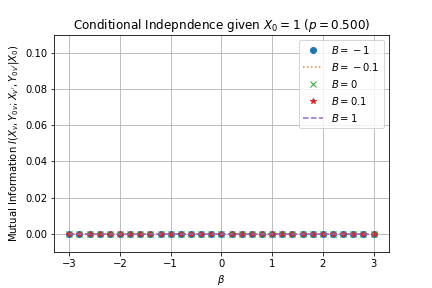
\includegraphics[width=7.5cm]{img/EA_x1_x2_x0=1_3s_p=0.50_kappa=2.png}
    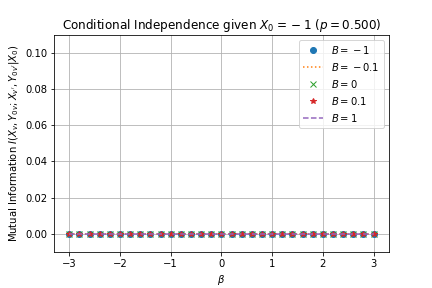
\includegraphics[width=7.5cm]{img/EA_x1_x2_x0=-1_3s_p=0.50_kappa=2.png}
    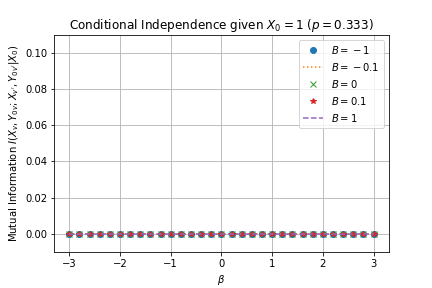
\includegraphics[width=7.5cm]{img/EA_x1_x2_x0=1_3s_p=0.33_kappa=2.png}
    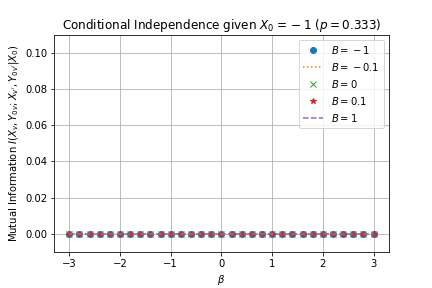
\includegraphics[width=7.5cm]{img/EA_x1_x2_x0=-1_3s_p=0.33_kappa=2.png}
    \caption{Edward-Anderson with edge marks $\{-1, 0, 1\}$ and $\kappa=2$. $\eta_Y(0)=p$ and $\eta_Y(-1)=\eta_Y(1)=\frac12(1-p)$. Edge-vertex marks are conditionally independent given the root mark.}
    \label{Fig.EA-CI-k2-3s}
\end{figure}

\newpage

Confirming with 5 states. We have $\mathcal{Y}=\{-2, -1, 0, 1, -2\}$ and $\eta_Y(0)=p$, $\eta_Y(\pm 1)=q$, $\eta_Y(\pm 2)=\frac12-\frac12p-q$

\begin{figure}[h]
    \centering
    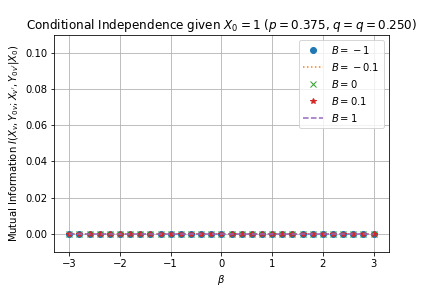
\includegraphics[width=7.5cm]{img/EA_x1_x2_x0=1_5s_p=0.38_q=0.25_kappa=2.png}
    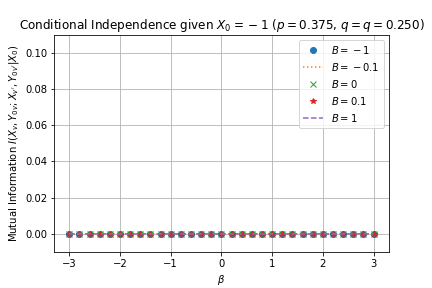
\includegraphics[width=7.5cm]{img/EA_x1_x2_x0=-1_5s_p=0.38_q=0.25_kappa=2.png}
    \caption{Edward-Anderson with edge marks $\{-2, -1, 0, 1, 2\}$ and $\kappa=2$. $\kappa=2$. $\eta_Y(0)=p$, $\eta_Y(\pm 1)=q$, $\eta_Y(\pm 2)=\frac12-\frac12p-q$. Edge-vertex marks are conditionally independent given the root mark.}
    \label{Fig.EA-CI-k2-5s}
\end{figure}

\newpage

\subsubsection{Root mark distribution}

We can see that for symmetric $\eta_Y$, we consistently get a root mark distribution independent on $\beta$. Again, we plot $\log\frac{\mu_0^+}{\mu_0^-}$:

\begin{figure}[h]
    \centering
    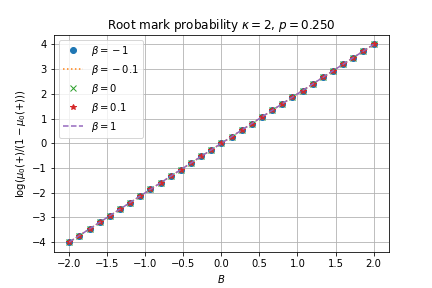
\includegraphics[width=7.5cm]{img/EA_x0_B_logi_kappa_2_3s_p=0.25.png}
    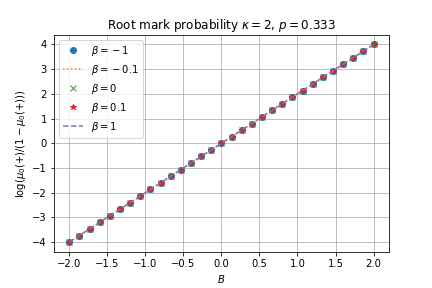
\includegraphics[width=7.5cm]{img/EA_x0_B_logi_kappa_2_3s_p=0.33.png}
    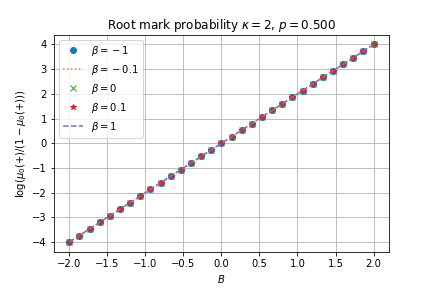
\includegraphics[width=7.5cm]{img/EA_x0_B_logi_kappa_2_3s_p=0.50.png}
    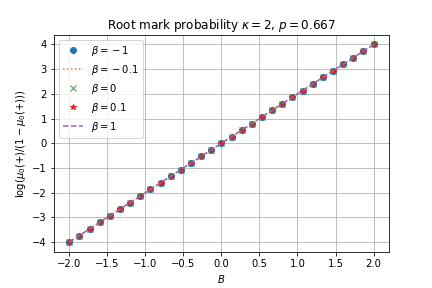
\includegraphics[width=7.5cm]{img/EA_x0_B_logi_kappa_2_3s_p=0.67.png}
    \caption{Edward-Anderson model with edge marks $\{-1, 0, 1\}$ and $\kappa=2$. $\eta_Y(0)=p$ and $\eta_Y(-1)=\eta_Y(1)=\frac12(1-p)$. The root mark distribution is independent of $B$}
    \label{Fig.EA-RM-k2-3s}
\end{figure}

\newpage

The conclusion is consistent with 5 edge states.
\begin{figure}[h]
    \centering
    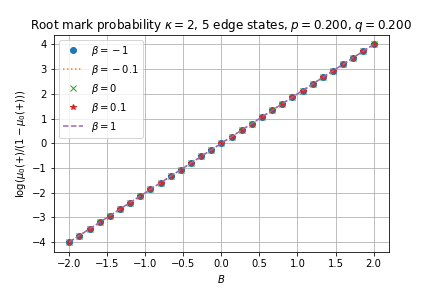
\includegraphics[width=7.5cm]{img/EA_x0_B_logi_kappa_2_5s_p=0.20_q=0.20.png}
    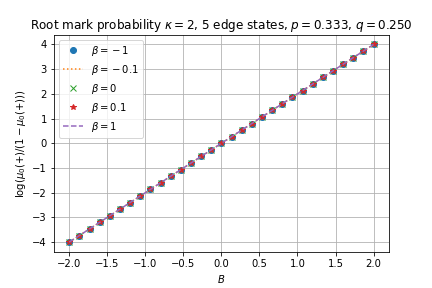
\includegraphics[width=7.5cm]{img/EA_x0_B_logi_kappa_2_5s_p=0.33_q=0.25.png}
    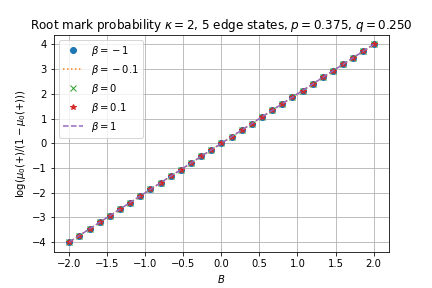
\includegraphics[width=7.5cm]{img/EA_x0_B_logi_kappa_2_5s_p=0.38_q=0.25.png}
    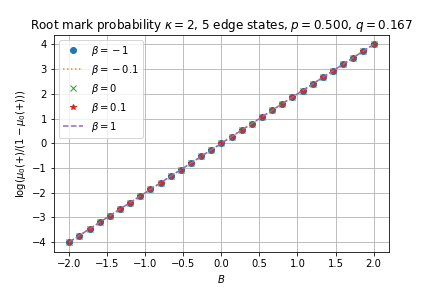
\includegraphics[width=7.5cm]{img/EA_x0_B_logi_kappa_2_5s_p=0.50_q=0.17.png}
    \caption{Edward-Anderson model with edge marks $\{-2, -1, 0, 1, -2\}$ and $\kappa=2$. $\eta_Y(0)=p$, $\eta_Y(\pm 1)=q$, $\eta_Y(\pm 2)=\frac12-\frac12p-q$. The root mark distribution is indepenident of $B$}
    \label{Fig.EA-RM-k2-5s}
\end{figure}

\newpage
The conclusion does not change with more leaves:
\begin{figure}[h]
    \centering
    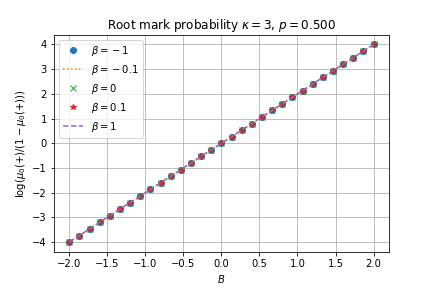
\includegraphics[width=7.5cm]{img/EA_x0_B_logi_kappa_3_3s_p=0.50.png}
    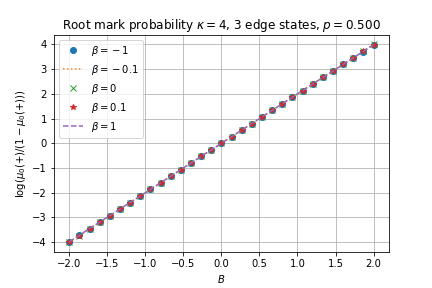
\includegraphics[width=7.5cm]{img/EA_x0_B_logi_kappa_4_3s_p=0.50.png}
    \caption{Edward-Anderson model with edge marks $\{-1, 0, 1\}$ and $\kappa=3$. $\eta_Y(0)=p$ and $\eta_Y(-1)=\eta_Y(1)=\frac12(1-p)$. The root mark distribution is independent of $B$}
    \label{Fig.EA-RM-k3-3s}
\end{figure}

Recall that in Ising model, we have a cavity field term that makes the root mark distribution dependent on $\beta$. Why is it the case that by adding
an edge mark makes this term disappear? We notice that Ising model is equivalent to Edward-Anderson with $\eta_Y=\delta_1$. This is not a symmetric
distribution. This leads to the hypothesis that a non-symmetric $\eta$ leads to a root-mark distribution dependent on $\beta$.

We instead consider a more general form of symmetry: $\eta_Y(\bar{Y}+\Delta y) = \eta_Y(\bar{Y}-\Delta y)$, still with evenly-spaced $\mathcal{Y}$.
\begin{figure}[h]
    \centering
    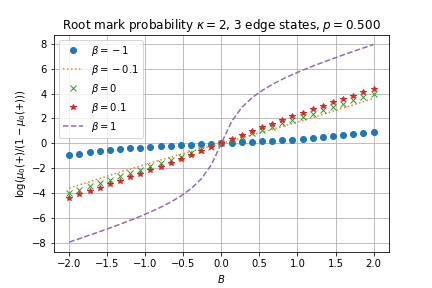
\includegraphics[width=10cm]{img/EA_x0_B_logi_kappa_2_3s_p=0.50_symF.png}
    \caption{Edward-Anderson model with edge marks $\{0, 1, 2\}$, $\eta_Y(1)=p$ and $\eta_Y(0)=\eta_Y(2)=\frac12(1-p)$. We see that the root mark distribution is now dependent on $\beta$}
    \label{Fig.EA-RM-k2-3s-asym}
\end{figure}

\newpage

\section{Jul 10-14}

\subsection{Hardcore Ising Numerical}
We now have Hamiltonian
\begin{equation}
    \mathcal{H}(x_0, k) = \beta x_0
\end{equation}
with constraint that
\begin{equation}
    \mu(x_0, k) = 0 \qquad \forall x_0=1, k>0
\end{equation}
The optimization target is the same:
\begin{equation*}
    \mathbb{E}_\mu[\beta X_0] - H(\mu \| \eta) + \frac\kappa2 H(\pi_\mu \| \pi_\eta)
\end{equation*}

For the optimizer, it is easier to deal with a smaller vector and assume the rest are simply 0.
\begin{equation*}
    (\mu_{-0}, \mu_{-1}, \cdots, \mu_{-\kappa}, \mu_{+0})
\end{equation*}

\subsubsection{Conditional Independence}

We observe conditional independence given root mark on small $\kappa$ values:
\begin{figure}[h]
    \centering
    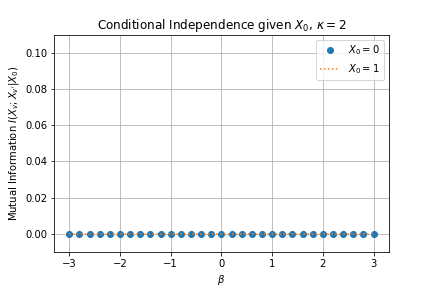
\includegraphics[width=7.5cm]{img/HA_Ising/CI_kappa2.png}
    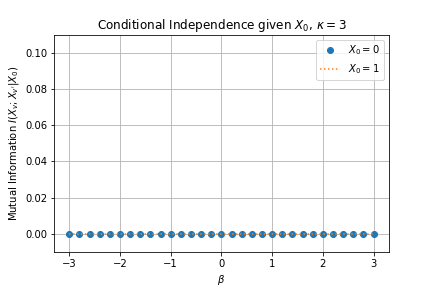
\includegraphics[width=7.5cm]{img/HA_Ising/CI_kappa3.png}
    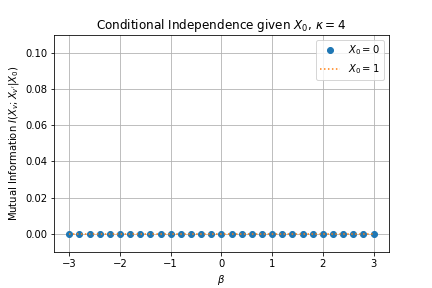
\includegraphics[width=7.5cm]{img/HA_Ising/CI_kappa4.png}
    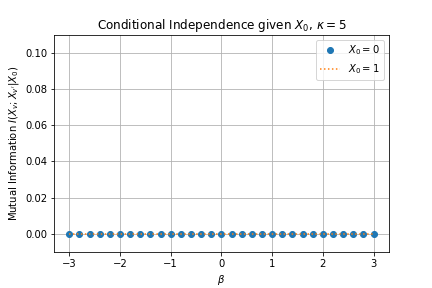
\includegraphics[width=7.5cm]{img/HA_Ising/CI_kappa5.png}
    \caption{In Hardcore Ising model, we still observe conditional independence for $\kappa=2, 3, 4, 5$.}
    \label{Fig.HAIS-CI}
\end{figure}

The conclusion is not changed for higher $\kappa$ values:
\begin{figure}[h]
    \centering
    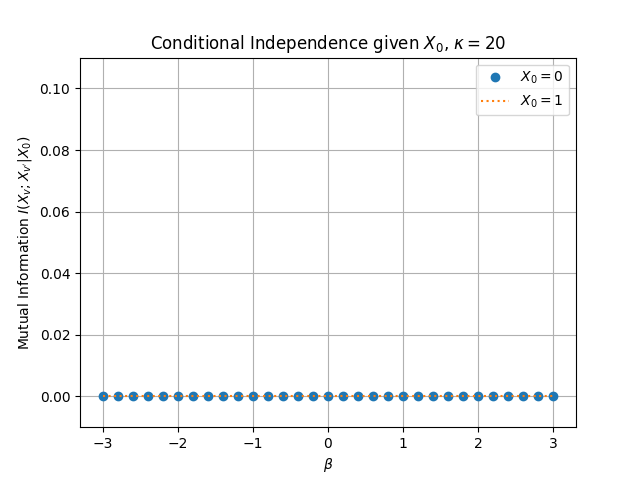
\includegraphics[width=8cm]{img/HA_Ising/CI_kappa20.png}
    \caption{In Hardcore Ising model, we still observe conditional independence for $\kappa=20$.}
    \label{Fig.HAIS-CI-large-kappa}
\end{figure}

\subsubsection{Root mark distribution}

This is the root mark distribution of Hardcore Ising
\begin{figure}[h]
    \centering
    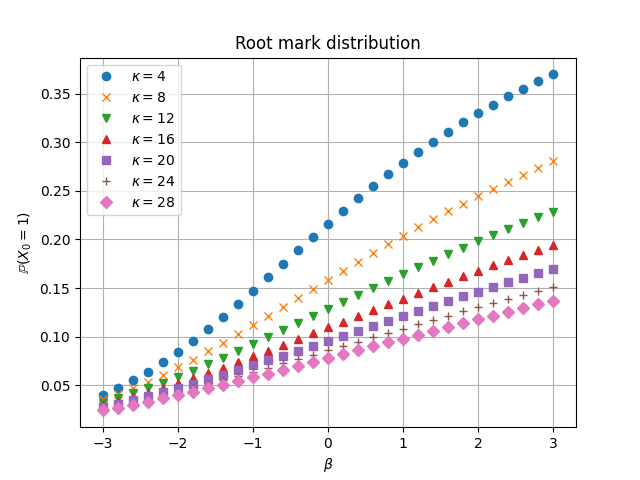
\includegraphics[width=10cm]{img/HA_Ising/RM_raw.png}
    \caption{This is the Root mark distribution for Hardcore Ising model. No significant transition is seen at $\kappa=16$}
    \label{Fig.HAIS-RM}
\end{figure}

\newpage

\subsubsection{Edge Distribution}

We see that the root and leaf marks ($\pi_\mu$) are never independent, and only tends to a degenerate independence as $\beta\rightarrow-\infty$.
\begin{figure}[h]
    \centering
    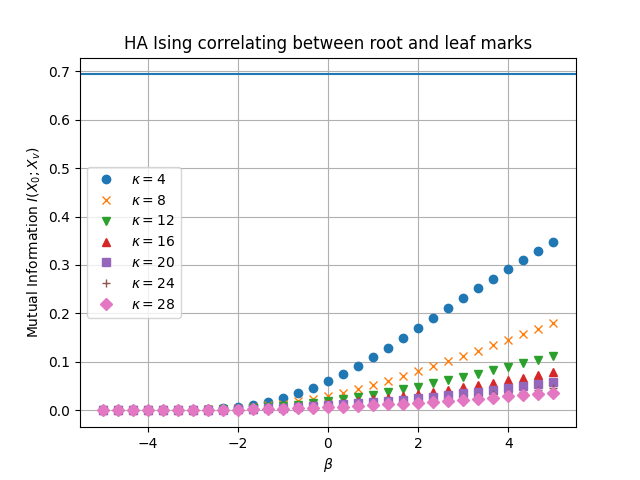
\includegraphics[width=10cm]{img/HA_Ising/RL_indep.png}
    \caption{In Hardcore Ising, $X_0$ and $X_v$ tends to independence as $\beta\rightarrow-\infty$, and they tend towards dependence as $\beta\rightarrow\infty$. The top line is at $\log 2$, the maximum mutual information possible with Bernoulli random variables.
        It is when $X_0$ are completely dependent on each other ($X_0=f(X_v)$).}
    \label{Fig.HAIS-RL-indep}
\end{figure}

To see what type of dependence we have, we look at the $\pi_\mu$ distribution:
\begin{figure}[h]
    \centering
    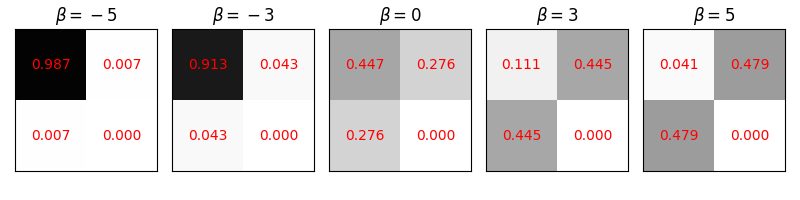
\includegraphics[width=15cm]{img/HA_Ising/RL_indiv.png}
    \caption{$\pi_\mu$ distribution under different $\beta$ values in Hardcore Ising ($\kappa=2$) is shown. Darker means greater value. $X_0=0$ is the top row and $X_v$ is the left column.}
    \label{Fig.HAIS-RL-beta-trends}
\end{figure}

First observe that due to the symmetry constraint, the $\pi_\mu$ distribution is represented by a symmetric matrix. Then, see that $\pi_\mu(1, 1)$ has $0$ probability due to the hardcore constraint.

When $\beta\rightarrow-\infty$, we observe that the distribution tends to have $X_0=X_v=0$. Indeed, this tends towards independence, but it is more
degenerate. When $\beta\rightarrow\infty$, we see that it tends towards $X_0=1-X_v$, preferring the root and leaves to have different marks.
Mark distributions also tend towards Bernoulli(1/2) (Due to the symmetry constraint).

\newpage

\subsection{Hardcore Ising Analytical}

\subsubsection{Conditional Independence}

Similar to what we have been doing, we can write the objective function as
\begin{equation*}
    V = \beta\sum_{x\in\mathcal{X}} \mu_0(x) x + H(\mu) + \sum_{x\in\mathcal{X}}\sum_{k=0}^\kappa \mu(x, k)\log{\kappa\choose k} - \frac\kappa2 H(\pi_\mu) - \log|\mathcal{X}|
\end{equation*}
where $\mu_0(x) = \sum_{k=0}^\kappa\mu(x, k)$.

Solving for this optimization problem (over hardcore support) with constraints
$\pi_\mu(0, 0) = \frac1\kappa\sum_{k=0}^\kappa k\mu(0, k) = \pi_\mu^-$, $\sum_{x\in\mathcal{X}}\sum_{k=0}^\kappa \mu(x, k)=1$, and $\mu_0(1) - \mu_0(0) = m$, we have the following form for $\mu$:
\begin{equation}
    \begin{cases}
        \mu(0, k) & = \displaystyle\frac{e^{-\gamma}(1+q^-)^\kappa}{e^\gamma + e^{-\gamma}(1+q^-)^\kappa}{\kappa\choose k}\left(\frac{q^-}{1+q^-}\right)^k\left(\frac{1}{1+q^-}\right)^{\kappa-k} \\
        \mu(1, 0) & = \displaystyle\frac{e^{\gamma}}{e^\gamma + e^{-\gamma}(1+q^-)^\kappa}
    \end{cases}
\end{equation}
where $\log q^-$ and $\gamma$ are the Lagrange multipliers to $\pi_\mu(0, 0) = \frac1\kappa\sum_{k=0}^\kappa k\mu(0, k) = \pi_\mu^-$ and $\mu_0(1) - \mu_0(0) = m$ respectively.

Applying the symmetry constraint, we have
\begin{equation}
    e^\gamma = e^{-\gamma}(1+q^-)^{\kappa-1}
\end{equation}
This gives
\begin{equation}
    \begin{cases}
        \mu(0, k) & = \displaystyle\frac{1+q^-}{2+q^-}{\kappa\choose k}\left(\frac{q^-}{1+q^-}\right)^k\left(\frac{1}{1+q^-}\right)^{\kappa-k} \\
        \mu(1, 0) & = \displaystyle\frac{1}{2+q^-}
    \end{cases}
    \label{Eq.HAIS-Q-SOL}
\end{equation}

\subsubsection{Solving for parameters}

We therefore need to optimize
\begin{equation*}
    \sup_{\pi_\mu^-\in(0, 1)}\left[ \mathbb{E}_{\mu_0} \beta X_0 + \frac\kappa2 H(\pi_\mu) - (\kappa-1) H(\mu_0) \right]
\end{equation*}
where $\mu_0(x_0) = \sum_{x_v\in\mathcal{X}}\pi_\mu(x_0, x_v)$. We can write $\pi_\mu(1, 0) = \pi_\mu(0, 1) = \frac12(1 - \pi_\mu^-)$

Applying Lagrange multiplier
\begin{equation}
    \partial_{\pi_\mu^-} = -\frac\beta2-\frac\kappa2 \left[\log\pi_\mu^- - \log \frac12(1 - \pi_\mu^-)\right] - \frac{\kappa-1}{2}\log\frac{1-\pi_\mu^-}{1+\pi_\mu^-} = 0
\end{equation}
If we substitute $\pi_\mu^-=\frac{q^-}{2+q^-}$, which can be obtained from (\ref{Eq.HAIS-Q-SOL}), we have
\begin{equation*}
    \beta + \kappa \log q^- - (\kappa-1)\log (1+q^-) = 0
\end{equation*}
or
\begin{equation}
    \frac{1}{1+q^-} = e^\beta \left(\frac{q^-}{1+q^-}\right)^\kappa
\end{equation}
We can then calculate the root mark distributions:
\begin{align}
    \mu_0(0) & = \frac{1+q^-}{2+q^-} = \frac{1}{1+\frac{1}{1+q^-}}  \nonumber          \\
             & = \frac{1}{1 + e^\beta \left(\frac{q^-}{1+q^-}\right)^\kappa} \nonumber \\
             & = \frac{(1+q^-)^\kappa }{(1+q^-)^\kappa + e^\beta (q^-)^\kappa}
    \intertext{Similarly, }
    \mu_0(1) & = \frac{e^\beta (q^-)^\kappa}{(1+q^-)^\kappa + e^\beta (q^-)^\kappa}
\end{align}
We then have distribution
\begin{equation*}
    \begin{cases}
        \mu(0, k) = \displaystyle\frac{1}{(1+q^-)^\kappa + e^\beta (q^-)^\kappa}{\kappa\choose k} (q^-)^k \\
        \mu(1, 0) = \displaystyle\frac{e^\beta (q^-)^\kappa}{(1+q^-)^\kappa + e^\beta (q^-)^\kappa}
    \end{cases}
\end{equation*}
Alternatively, writing $q^- = \exp h$,
\begin{equation}
    \begin{cases}
        \mu(0, k) = \frac1Z{\kappa\choose k} e^{kh} \\
        \mu(1, 0) = \frac1Z e^{\beta + \kappa h}
    \end{cases}
\end{equation}
where $Z = (1+e^h)^\kappa + e^{\beta + \kappa h}$.

More concisely,
\begin{equation}
    \mu(\mathbf{x}, \tau) = \frac1Z \exp\left[\beta x_0 + h \sum_{v\in\mathcal{N}_o(\tau)}(1-x_v)\right]
\end{equation}
where $h = (\kappa - 1)\log (1+e^{-h}) - \beta $

\newpage

\subsection{Cross Reference}

We will now check the analytical results to the numerical results. Note that
\begin{equation*}
    h = \log\frac{1 - 2 \mu_0(1)}{\mu_0(1)}
\end{equation*}
From data gathered in Fig.\ref{Fig.HAIS-RM}, we see that the analytical results agree with numerical
\begin{figure}[h]
    \centering
    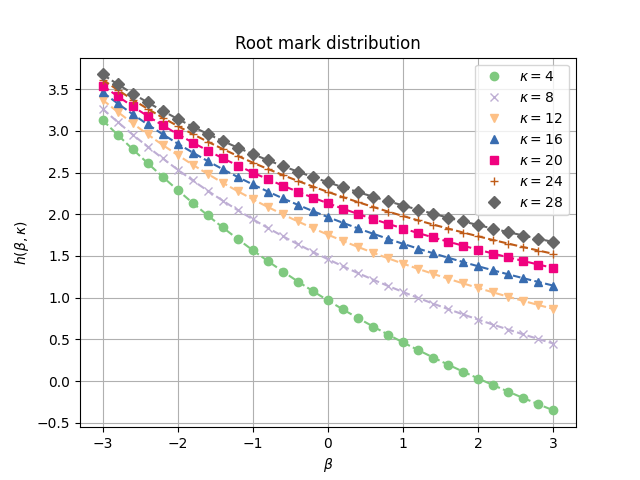
\includegraphics[width=10cm]{img/HA_Ising/h_value.png}
    \caption{Hardcore Ising, comparison of numerical and analytical predictions of $h$. The dashed lines show analytical predictions.}
    \label{Fig.HAIS-h-value}
\end{figure}

Regarding the edge distribution, we first notice that when $\beta\rightarrow\infty$, $h\rightarrow -\infty$, and when $\beta\rightarrow-\infty$, $h\rightarrow \infty$ (Desmos).

We write $\pi_\mu$ in terms of $h$:
\begin{align*}
    \pi_\mu(0, 0)                 & = \frac{1}{2e^{-h} + 1} \\
    \pi_\mu(1, 0) = \pi_\mu(0, 1) & = \frac{1}{2+e^h}
\end{align*}
When $\beta\rightarrow\infty$, $h\rightarrow-\infty$, so $\pi_\mu(0, 0)\rightarrow 0$, and $\pi_\mu(1, 0) = \pi_\mu(0, 1)\rightarrow \frac12$.

When $\beta\rightarrow-\infty$, $h\rightarrow\infty$, so $\pi_\mu(0, 0)\rightarrow 1$, and $\pi_\mu(1, 0) = \pi_\mu(0, 1)\rightarrow 1$.

This agrees with our predictions in Fig.\ref{Fig.HAIS-RL-beta-trends}.

\end{document}